%%%%%%%%%%%%%%%%%%%%%%%%%%%%%%%%%%%%%%%%%%%%%%%%%%%%%%%%%%%%%%%%%%%%%%%%%%%%%%%
%  Heimdall: Discovering IPv6 Fully-Responsive Prefixes at Scale via
%  Dual-Scan Hierarchical State-Space Models with In-Range-Aware Feedback
%
%  Target venue : IEEE INFOCOM 2027
%  Template     : IEEEtran conference (double-column, 10pt)
%
%  How to build:
%      pdflatex Heimdall_infocom2027 && bibtex Heimdall_infocom2027 && \
%      pdflatex Heimdall_infocom2027 && pdflatex Heimdall_infocom2027
%
%  Figures required in the same directory:
%      frp_count.pdf          address_space.pdf
%      as_coverage.pdf        country_coverage.pdf
%      prefix_coverage.pdf    category_coverage.pdf
%      comparison_curves.pdf  (optional, used for the summary figure)
%      arch_dualscan.pdf      (system overview — TBD)
%      seed_overlap.pdf       (raw vs net-new FRPs at 10M budget)
%      netnew_curve.pdf       (net-new FRPs across budgets)
%%%%%%%%%%%%%%%%%%%%%%%%%%%%%%%%%%%%%%%%%%%%%%%%%%%%%%%%%%%%%%%%%%%%%%%%%%%%%%%
\documentclass[conference]{IEEEtran}
\IEEEoverridecommandlockouts
\usepackage{cite}
\usepackage{amsmath,amssymb,amsfonts}
\usepackage{algorithm}
\usepackage{algpseudocode}
\usepackage{graphicx}
\usepackage{textcomp}
\usepackage{xcolor}
\usepackage{booktabs}
\usepackage{multirow}
\usepackage{url}
\usepackage{hyperref}
\usepackage{siunitx}
\usepackage[skip=2pt,belowskip=-4pt,font=small,labelfont=bf]{caption}
\usepackage[skip=1pt,font=footnotesize]{subcaption}
\hypersetup{colorlinks=true,linkcolor=blue,citecolor=blue,urlcolor=blue}

\def\BibTeX{{\rm B\kern-.05em{\sc i\kern-.025em b}\kern-.08em
             T\kern-.1667em\lower.7ex\hbox{E}\kern-.125emX}}

\begin{document}

\title{Heimdall: Discovering IPv6 Fully-Responsive Prefixes at Scale via
       Dual-Scan Hierarchical State-Space Models with In-Range-Aware
       Feedback}

\author{
% \IEEEauthorblockN{Yuchen Gu\IEEEauthorrefmark{1},
% Lin He\IEEEauthorrefmark{2},
% Ying Liu\IEEEauthorrefmark{2}}
}

\maketitle

% =============================================================================
%  Abstract
% =============================================================================
\begin{abstract}
Fully Responsive Prefixes (FRPs)---IPv6 prefixes where every address replies to probes---are critical for Internet-wide measurement and target generation, yet exhaustive discovery is impossible in the 128‑bit address space. 
Leading generators, \emph{Luori} and \emph{Gungnir}, either concentrate their probing budget within a handful of Autonomous Systems (ASes) or waste a large fraction of it on candidates \emph{already covered by the known seed set}. 
We show that $32\%$--$43\%$ of the FRPs confirmed by these generators are strict sub‑prefixes of the aligned public seed set, contributing no fresh information. 
We present \textbf{Heimdall}, an online FRP discovery framework built around a \emph{Dual‑Scan Hierarchical Mamba} (DS‑HMamba) generator. 
DS‑HMamba jointly performs an \emph{outer scan} over the 128‑bit address hierarchy and an \emph{inner scan} across samples from the same AS, fused by an AS‑conditioned gate. 
Candidates are validated by a ping‑style probing module, and Heimdall excludes any candidate already covered by a known FRP, so that every probe seeks \emph{net‑new} prefixes; the resulting labels then continually fine‑tune DS‑HMamba. 
Under identical budgets of 2--10\,M packets, Heimdall discovers $\mathbf{2.8\times}$ more raw and $\mathbf{3.23\times}$ more net‑new FRPs than Gungnir, covers $\mathbf{5.9\times}$ more address space and $\mathbf{3.2\times}$ more ASes.
\end{abstract}

\begin{IEEEkeywords}
IPv6 measurement, Fully-Responsive Prefix, Address-space discovery,
Hierarchical state-space model, Mamba, Active probing, Online
learning.
\end{IEEEkeywords}


% =============================================================================
%  I.  Introduction
% =============================================================================
\section{Introduction}\label{sec:intro}

Internet-wide active scanning underpins modern Internet
measurement~\cite{durumeric2013zmap,rye2023ipv6hitlist,foremski2016entropy,pour2020comprehensive,durumeric2013zmap-ext,google-v6-stats}.
While IPv4 has been mapped in its
entirety~\cite{durumeric2013zmap,zgrab2}, the $2^{128}$ address space of IPv6
renders brute-force scanning infeasible and has motivated numerous Target Generation Algorithms
(TGAs)~\cite{song2022det,yang20226forest,hou20216hit,zhang20246vision,zhou20236tree-ml,song2020hitlist,liu20166tree,song20206gcvae,song20216veclm,song20216gan,yang20226graph,liu2018build-hitlist}.
These TGAs are, however, undermined by a peculiar phenomenon: a
significant portion of the addressable space consists of
\emph{Fully Responsive Prefixes} (FRPs)--- prefixes where
\emph{every} address responds to
probes~\cite{gasser2018clusters,zirngibl2022rusty,sattler2023hrp,cheng2024luori,cheng2024seed-selection,plonka2015temporal}.
FRPs distort measurement conclusions (hitlist inflation, service
counts, reachability), waste bandwidth and complicate downstream
analyses~\cite{erdemir2025aliases,gharaibeh2017look,li2022fast6,vermeulen2020multilevel,vermeulen2020diamond,eddy2007synflood}.  Discovering them precisely is
therefore a first-class problem for the research community.

Two recent efforts represent the state of the art.
\emph{Luori}~\cite{cheng2024luori} casts FRP discovery as a
reinforcement-learning problem and expands a prefix tree via
Monte-Carlo Tree Search.  \emph{Gungnir}~\cite{wei2025gungnir}
introduces a Transformer autoregressive model that unifies multiple
protocols and applies a granularity-correction post-process.  Both
methods, however, share three limitations that we systematically
diagnose in this paper.
First, neither method excludes candidates that fall \emph{inside} an
already-known FRP range at generation time (\textbf{redundancy
w.r.t.\ the known range}): in our large-scale reproduction, under a
$10$M probing budget $43\%$ of Gungnir's confirmed FRPs are strict
sub-prefixes of the aligned public seed set and $32\%$ of Luori's
are, so the corresponding probes contribute no fresh signal (a sub-prefix of a known FRP is fully responsive by definition) (\S\ref{sec:redundancy}).
Second, Transformer decoders treat each prefix in isolation (\textbf{weak intra-AS coupling}), yet FRPs from a single AS share nibble-level patterns (\S\ref{sec:motivation}); ignoring these correlations forces the model to re-discover repeated substructures.
Third, both baselines are frozen after training (no online feedback), and thus cannot adapt to real-world dynamics (churn, new allocations).

To this end, we propose \textbf{Heimdall}, an online FRP discovery
framework whose core idea is to restrict probing to prefixes
outside the aligned public seed set---referred to as \emph{net‑new} discoveries---and continuously adapt the
generator through online feedback.  Heimdall consists of
\textbf{four modules} arranged as a closed feedback loop
(Fig.~\ref{fig:arch}):
\emph{(i)}~a \textbf{DS-HMamba generator}
(\S\ref{sec:design:model}) that combines an \emph{outer scan}
over the 128-bit address hierarchy with an \emph{inner scan} over
same-AS samples, fused by an AS-conditioned gate to jointly
exploit intra-prefix and intra-AS regularities;
\emph{(ii)}~a three-stage \textbf{MLM decoder head}
(\S\ref{sec:design:decoder}) that shares parameters with the
generator and turns its representation into concrete candidates
via coarse-to-fine temperature-controlled top-$p$ sampling;
\emph{(iii)}~a \textbf{SeedFilter}
(\S\ref{sec:design:seedfilter}) that pre-fixes the known-FRP
set at start-up and rejects every candidate covered by it,
ensuring each probe seeks a net-new prefix;
\emph{(iv)}~an \textbf{active prober plus online fine-tuner}
(\S\ref{sec:design:prober}--\ref{sec:design:tuner}) that
verifies survivors with a robust APD variant and feeds
confirmed / rejected labels back to DS-HMamba, closing the
in-range-aware feedback loop.

\smallskip\textbf{Contributions.}
The primary contributions of this work are as follows:
\begin{itemize}
    \item We are the first, to the best of our knowledge, to
    quantify the \emph{in-range redundancy} of state-of-the-art FRP
    generators and to show that Gungnir spends $43\%$ of its confirmed
    hits (and Luori $32\%$) on candidates strictly inside the aligned
    seed range (\S\ref{sec:redundancy}).
    \item We propose DS-HMamba, a dual-scan hierarchical state-space
    model that jointly exploits the intra-prefix bit hierarchy and
    the intra-AS sample correlations at $O(L)$ time per layer,
    strictly cheaper than the $O(L^2)$ self-attention used by
    Gungnir (\S\ref{sec:design:model}).
    \item We design a two-level SeedFilter and an in-range-aware
    online fine-tuning loop that turns wasted probes into productive
    discovery (\S\ref{sec:design:seedfilter}--\ref{sec:design:tuner}).
    \item Under identical 2\,M--10\,M probing budgets on the
    public IPv6 routing view, Heimdall outperforms Gungnir by up to
    \textbf{2.8$\times$} on raw confirmed FRPs and
    \textbf{3.23$\times$} on net-new confirmed FRPs;
    \textbf{5.9$\times$} on covered address space; \textbf{3.2$\times$}
    on ASes and \textbf{1.76$\times$} on countries.  Against Luori
    the net-new gap is $\mathbf{1.35\times}$ at $10$M and grows
    monotonically with the budget (\S\ref{sec:eval:perf}).
\end{itemize}


% =============================================================================
%  II.  Background and Related Work
% =============================================================================
\section{Background and Related Work}\label{sec:background}

\subsection{Fully Responsive Prefixes}
Murdock \emph{et al.}~\cite{murdock2017tga} first noticed the
misleading effect of \emph{aliased prefixes}---contiguous IPv6
ranges whose addresses reply uniformly to probes---on address
inference.  Zirngibl \emph{et al.}~\cite{zirngibl2022rusty} refined
the definition and adopted the term FRP, formally requiring a
$100\%$ probe-reply rate across the prefix.  Sattler \emph{et
al.}~\cite{sattler2023hrp} report similar aliasing-driven inflation.
Their operational relevance is now well-established: FRPs distort
hitlists~\cite{gasser2018clusters,steger2023tga,plonka2015temporal},
inflate service counts and complicate downstream
analyses~\cite{erdemir2025aliases}.

\subsection{FRP Probing}
\label{sec:bg:probing}
\subsubsection{Aliased Prefix Detection (APD) and MAPD}
The seminal APD proposed by Gasser \emph{et al.}~\cite{gasser2018clusters}
probes $16$ addresses, one per nibble, drawn from the sixteen child
\texttt{0}--\texttt{f} sub-prefixes of a candidate prefix; if all $16$ addresses respond, the prefix is classified as aliased.  Its exhaustive variant,
MAPD~\cite{zirngibl2022rusty}, enumerates all parent prefixes down
to prefix length $\ell{=}64$. However, its probing cost grows exponentially with the announced
prefix length, making it infeasible under a bounded probing budget.

\subsubsection{Luori~\cite{cheng2024luori}}
\label{sec:bg:luori}
It casts FRP discovery as a Monte-Carlo Tree Search
(MCTS)~\cite{silver2016mcts} problem, borrowing the UCB strategy
from AlphaGo.  It builds a prefix tree rooted at each routing
prefix and lets an MCTS agent decide, at every internal node,
which child sub-prefix to expand next; the reward comes from
the outcome of an APD probe applied at the reached leaf, and a
reinforcement learning policy learns to prioritize sub-trees
rich in FRP density.  Luori's design is elegant but inherits
three well-documented weaknesses of tree-based RL.
\emph{(i)~Length dependency.}  Every path in the tree must be
expanded bit-by-bit, so the effective search depth grows
linearly with prefix length; large announcements (e.g.\ /32)
exhaust the sampling budget long before the tree is developed.
\emph{(ii)~Local exploitation.}  MCTS concentrates rollouts on
sub-trees that already contain confirmed FRPs; consequently,
Luori quickly rediscovers a rich sub-space around the seed and
then saturates (this behaviour is visible in
Fig.~\ref{fig:panels_raw}(a), where Luori's raw FRP count
flattens between $8$M and $10$M).
\emph{(iii)~No cross-AS transfer.}  Trees for different routing
prefixes do not share statistics, so patterns common to an
entire AS or business category must be re-learned from scratch
every time.

\subsubsection{Gungnir~\cite{wei2025gungnir}}
\label{sec:bg:gungnir}
Gungnir is the most recent Transformer-based FRP generator.
Its multi-head self-attention backbone follows the standard
formulation of Vaswani \emph{et al.}~\cite{vaswani2017attention}
and the causal left-to-right decoding of
GPT-2~\cite{radford2019gpt2}.  It reformulates FRP discovery as
\emph{sequence modelling}: an IPv6 prefix is tokenised bit-by-bit
into a token sequence together with side tokens for BGP prefix,
AS, organisation, business category and protocol.  A Transformer
decoder with $N$ stacked Multi-Head-Self-Attention (MHSA) blocks
then learns the joint distribution
$P_\theta(w_1,\ldots,w_L\mid\text{ctx})$ under a causal
cross-entropy loss.  At inference time, candidates are generated
through a Markov chain of conditional probabilities, with
\emph{Top-$p$ nucleus sampling}~\cite{holtzman2020top-p}
controlling the exploration/exploitation trade-off (best
$p{=}0.6$).  After a candidate is confirmed by APD, Gungnir
performs \emph{granularity correction}: it re-probes the
candidate under alternative prefix lengths and keeps the largest
one that still yields $16/16$ replies, fighting the
\emph{FRP-misleading} effect where a smaller nested FRP is
reported instead of its actual container.  We identify three
structural weaknesses that motivate our paper: (i)~$43\%$ of
confirmed FRPs at $10$M are in-range w.r.t.\ the aligned public
seed set (\S\ref{sec:redundancy}); (ii)~$O(L^2)$ attention makes
Gungnir $1.7\!-\!2.1\times$ slower per candidate than a linear
scanner (\S\ref{sec:eval:resource}); (iii)~the model is frozen
after pre-training, so the redundancy ratio stays at
$\sim\!43\%$ across the entire budget grid.

\subsection{Selective State-Space Models}
\label{sec:bg:mamba}
Mamba~\cite{gu2023mamba,gu2021s4} is a recent \emph{selective}
State-Space Model (SSM) that reaches Transformer-level accuracy
at \emph{linear} time and memory in the sequence length.  Its
recurrence is
\begin{equation}
h_t = \exp(\Delta_t A)\,h_{t-1} + \Delta_t B_t u_t,
\quad y_t = C_t^{\top} h_t,
\label{eq:mamba-ssm}
\end{equation}
where the state matrix $A\!\in\!\mathbb{R}^{N\times N}$ is
diagonal and $(\Delta_t,B_t,C_t)$ are \emph{input-dependent}
gates that let the model selectively remember or forget along
the scan axis.  Because $A$ is diagonal and the update is a
first-order recurrence, the whole sequence can be evaluated by
a parallel prefix scan in $O(L\log L)$ work and $O(L)$ memory
--- an order of magnitude cheaper than attention on long
sequences.  Mamba has been successfully applied to language,
vision, audio and genomics, but --- to our knowledge --- has
not yet been used for IPv6 measurement.  We argue in
\S\ref{sec:design:why-mamba} that its linear-in-length cost and
selective-recurrence property are a strong match for FRP
generation.


% =============================================================================
%  III.  Problem Analysis and Motivation
% =============================================================================
\section{Problem Analysis and Motivation}\label{sec:motivation}

\subsection{Definitions}
\label{sec:motivation:def}
We work with three sets throughout.  Let
$\mathcal{S}\subset\{0,1\}^{\le128}\times\mathbb{N}$ denote the
current \emph{seed FRP set} (each entry is a prefix and its
routing length); let $\mathcal{S}_{0}\supseteq\mathcal{S}$
denote the \emph{aligned public seed set} obtained by unioning
$\mathcal{S}$ with third-party FRP releases and the APD-derived
aggregations described in \S\ref{sec:eval:setup}.  Given a
probing budget $B$ (in packets), $\mathcal{C}_\theta$ is the set
of candidate prefixes generated by algorithm $\theta$ and
$\mathcal{F}_\theta\!\subseteq\!\mathcal{C}_\theta$ the subset
whose APD test succeeds.  Because a probe that lands
\emph{inside} an already-known FRP $s\!\in\!\mathcal{S}_{0}$ can
only re-confirm what is known, we measure discovery quality by
the \emph{net-new coverage}
\begin{equation}
\mathrm{NN}(\theta) \;=\;
\big|\{c\in\mathcal{F}_\theta \,:\, \nexists\,s\in\mathcal{S}_{0},\;
   c\preceq s\}\big|,
\label{eq:netnew}
\end{equation}
where $c\preceq s$ means $c$ is a (non-strict) sub-prefix of $s$.
The corresponding \emph{redundancy ratio} of $\theta$ is
$\rho(\theta)\!=\!1-\mathrm{NN}(\theta)/|\mathcal{F}_\theta|$;
$\rho$ close to zero means every probe contributes new
information, while $\rho$ close to one means the generator merely
re-discovers what the community has already published.
Section~\ref{sec:redundancy} shows that state-of-the-art
generators sit at $\rho\!\approx\!0.32\!-\!0.43$.

\subsection{In-Range Probes Waste a Large Share of the Budget}
Under a $10$M packet budget Gungnir confirms $1{,}675$ FRPs, but a
full sub-prefix check against $\mathcal{S}_{0}$ (via
Eq.~(\ref{eq:netnew})) reveals that only $954$ are genuinely
\emph{net-new}; the remaining $721$ ($43.0\%$) fall inside a known
FRP.  Luori exhibits a milder but still material redundancy of
$31.9\%$ (Fig.~\ref{fig:seed_overlap}, dissected in
\S\ref{sec:redundancy}).  Two observations drive our design:
(a)~probing a sub-prefix of a known FRP is
\emph{information-free}: every $c\preceq s$ is fully responsive by
definition; and (b)~$\mathcal{S}_{0}$ is available \emph{before}
probing starts, so a $O(\log|\mathcal{S}_{0}|)$ trie lookup can
refuse redundant candidates.  Heimdall builds this lookup into a
two-level SeedFilter (\S\ref{sec:design:seedfilter}) that guarantees
every issued probe lands outside $\mathcal{S}_{0}$.

\subsection{FRPs Are Strongly Regular Within Each AS}
\label{sec:motivation:entropy}
Gungnir~\cite{wei2025gungnir} systematically measured the
\emph{pattern entropy}
$H_{\mathrm{pattern}}(\mathcal{S})=-\!\sum_x P(x)\log P(x)$
of the public FRP seed set at every prefix length, both globally
and after partitioning by business category, organisation and
announcing AS.  Their results establish two facts that we adopt
directly rather than re-measure: \emph{(i)}~all partitioned
curves sit far below the uniform-random upper bound, and the gap
widens monotonically as the partition becomes finer; and
\emph{(ii)}~for $\ell{=}20$ the observed entropy drops from
$\sim\!12.5$ (global) to $\sim\!5.2$ (top-1 AS), a $2.4\times$
compression, while the intra-AS residual is still non-trivial
(the model must exploit AS conditioning without collapsing to a
single per-AS template).

Two consequences follow for the generator design.  First, a
generator that models each prefix in isolation (as Gungnir does)
must re-derive intra-AS substructure from scratch, spending
$O(L^2)$ attention on an axis already exposed by the AS label.
Second, the intra-AS regularity motivates a \emph{second} scan
axis that runs across same-AS samples, learning the shared
nibble structures once.  This is the role of the \emph{inner
scan} in \S\ref{sec:design:model}.

\subsection{Goal}
Combining the two observations, we formalise Heimdall's design
objective as
\begin{equation}
\max_{\theta}\; \mathrm{NN}(\theta) \;\;
\text{s.t.}\;\; |\mathcal{C}_\theta|\!\le\!B/16,\;\;
c\not\preceq s\;\forall\,c\!\in\!\mathcal{C}_\theta,\,
s\!\in\!\mathcal{S}_{0},
\label{eq:obj}
\end{equation}
i.e.\ maximise net-new coverage subject to a probing budget
and the in-range exclusion constraint.  The next section
describes an architecture that fulfils both constraints
efficiently.


% =============================================================================
%  IV.  Design of Heimdall
% =============================================================================
\section{Design of Heimdall}\label{sec:design}

\subsection{Overview}\label{sec:design:overview}
Fig.~\ref{fig:arch} shows the pipeline of Heimdall.  The
\textbf{Seed Store} holds $\mathcal{S}_{0}$ and per-prefix
metadata, loaded once at start-up.  Four processing modules
follow on the main spine: the \textbf{DS-HMamba generator}
(\S\ref{sec:design:model}) with its \textbf{MLM decoder head}
(\S\ref{sec:design:decoder}) emits a $128$-bit candidate; the
\textbf{SeedFilter} (\S\ref{sec:design:seedfilter}) removes
duplicates and in-range candidates w.r.t.\ $\mathcal{S}_{0}$
\emph{before} probing; the \textbf{Active Prober}
(\S\ref{sec:design:prober}) verifies survivors with $16$ APD
probes; and the \textbf{Online Fine-tuner}
(\S\ref{sec:design:tuner}) refreshes DS-HMamba every
$\{0.5,2.5,4.5,6.5\}$\,M probes from confirmed and rejected
labels.  Compared to Luori (open-loop MCTS) and Gungnir
(open-loop autoregression), this is the first FRP architecture
whose generator is \emph{reactively adapted} to observed
outcomes.

\begin{figure*}[!t]
\centering
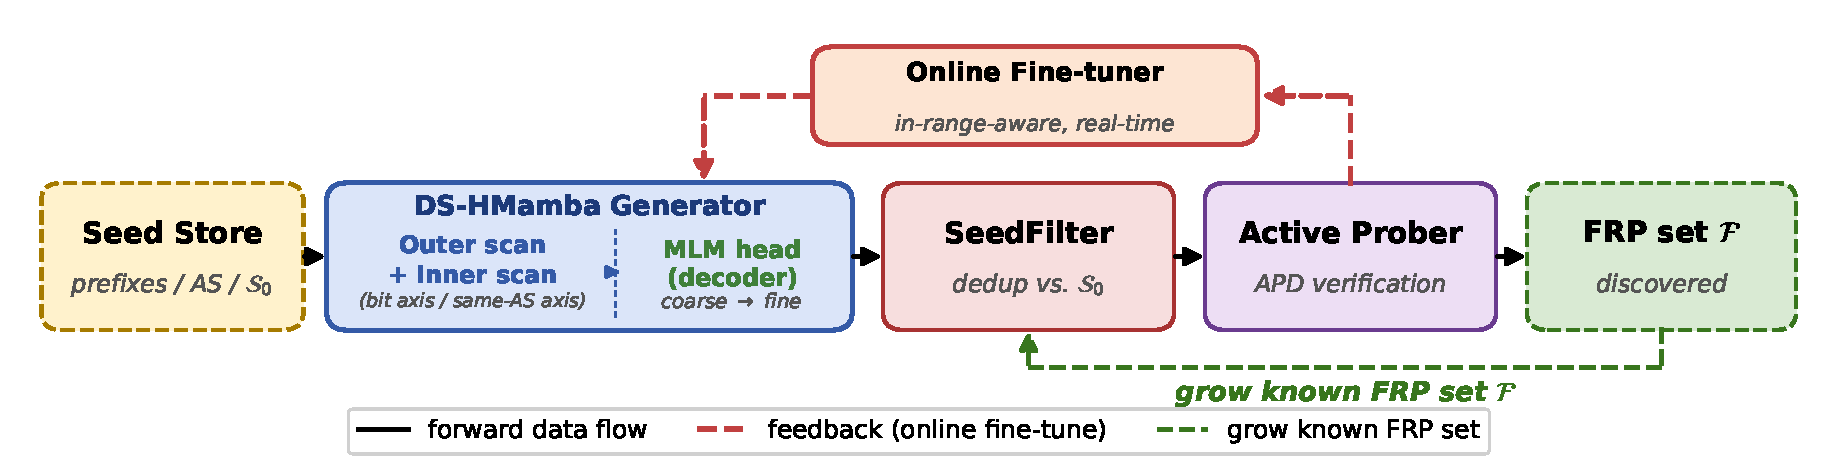
\includegraphics[width=\linewidth]{arch_dualscan.pdf}
\caption{Architecture of Heimdall.  Let $\mathcal{S}_{0}$
denote the public seed FRP set loaded at start-up
(\S\ref{sec:motivation:def}).  The four modules of
Sec.~\ref{sec:design} appear as boxes on the main spine and the
feedback lane: \textbf{DS-HMamba Generator}, \textbf{SeedFilter},
\textbf{Active Prober} and \textbf{Online Fine-tuner}.  Inside
the Generator, a sub-region marks the MLM decoder head, which
shares parameters with the dual-scan trunk and is therefore the
output layer of DS-HMamba rather than a separate module.  The
red dashed path is the in-range-aware feedback loop; the green
dashed path shows how confirmed FRPs grow $\mathcal{S}_{0}$
inside SeedFilter.}
\label{fig:arch}
\end{figure*}

\subsection{Design Rationale}
\label{sec:design:why-mamba}
The generator must satisfy four requirements dictated by the FRP
structure itself:
(\textbf{R1}) model long-range bit dependencies across all $L{=}128$
bits, since coarse bits (routing prefix, RIR block) constrain the
plausible medium and fine
bits~\cite{hinden2006rfc4291,deering1998ipv6};
(\textbf{R2}) run in $O(L)$ per layer, since a $10$M budget triggers
$\sim\!625$K generations and the $O(L^2)$ attention of Gungnir already
saturates a single RTX 4090
(Table~\ref{tab:ablation_resource}(b));
(\textbf{R3}) provide input-selective memory, because the effective
FRP alphabet is AS-dependent (some ASes have near-zero entropy on the
first eight nibbles, others carry information mostly in the fine bits;
\S\ref{sec:motivation:entropy});
and (\textbf{R4}) compose along a second axis running across
different prefixes of the same AS, since intra-AS samples share
nibble structures (\S\ref{sec:motivation:entropy}), without a
quadratic blow-up.
Mainstream architectures fail at least one: LSTM/GRU are $O(L)$
but their fixed recurrence cannot adaptively skip content
(fail R3) and struggle with very long contexts (weak on R1);
Transformer decoders address R1/R3 through attention but are
$O(L^2)$ (fail R2) and are not naturally composable along a
second axis (fail R4).  Selective State-Space Models
(Mamba~\cite{gu2023mamba,gu2021s4}) satisfy all four: the
recurrence in Eq.~(\ref{eq:mamba-ssm}) is $O(L)$ (R2); the
input-dependent gates $(\Delta_t,B_t,C_t)$ realise selective
memory (R3); the diagonal state matrix admits an efficient
parallel scan that generalises to a second axis (R4); and
empirically Mamba matches attention on retrieval-style tasks up
to $L{=}16$k tokens (R1).  We therefore adopt Mamba as the
backbone and compose two orthogonal scans on top of it.

\subsection{DS-HMamba Generator}
\label{sec:design:model}
DS-HMamba is the candidate-generation
core of Heimdall.  Given a target BGP prefix and its context
tokens (AS, organisation, business category, protocol), it
produces a probability distribution
$P_\theta(b_{1:L}\mid\text{ctx})$ over $128$-bit IPv6 prefixes
that the downstream MLM decoder (\S\ref{sec:design:decoder})
samples from.  Its job is therefore \emph{representation
learning}: turn a bit-hierarchical prefix plus its context into
a per-position feature tensor that jointly exploits (i)~the
coarse$\to$medium$\to$fine bit hierarchy and (ii)~the intra-AS
sample regularities revealed in \S\ref{sec:motivation:entropy}.

The module realises this role
through four functional stages executed in sequence:
bit-hierarchy embedding $\rightarrow$ outer scan (bit axis)
$\rightarrow$ inner scan (same-AS axis) $\rightarrow$
AS-conditioned gating fusion, described below.

\subsubsection{Bit-hierarchy embedding}An IPv6 prefix is a length-$L$ binary string
$b_{1:L}\!\in\!\{0,1\}^{L}$.  Motivated by
RFC~4291~\cite{hinden2006rfc4291}, we split the bit positions
into three semantic layers
\emph{coarse} $\mathcal{L}_c\!=\![1,\ell_c]$
(routing prefix + RIR block, typically $\ell_c\!=\!32$),
\emph{medium} $\mathcal{L}_m\!=\![\ell_c\!+\!1,\ell_m]$
(subnet allocation granularity, $\ell_m\!\approx\!48\text{--}64$),
and \emph{fine} $\mathcal{L}_f\!=\![\ell_m\!+\!1,L]$ (interface
identifier / suffix).  A learned bit-embedding lifts $b_i$ to
$x_i\!\in\!\mathbb{R}^{d}$ and each token receives an additive
layer embedding $e_s\!\in\!\{e_c,e_m,e_f\}$ so that the model
can distinguish coarse-medium-fine positions.

\subsubsection{Outer scan (bit axis)}
The outer scan is a stack of $N_o$ Mamba blocks operating on
the bit sequence $x_{1:L}$.  Each block executes the selective
SSM update of Eq.~(\ref{eq:mamba-ssm}), interleaved with a
gated Conv-1D of width $4$ and a residual FFN, closely
following the original Mamba block.  The output is a length-$L$
context tensor
$y^{\text{outer}}\!\in\!\mathbb{R}^{L\times d}$.  The outer
scan captures the
\emph{coarse$\rightarrow$medium$\rightarrow$fine} hierarchy of
an IPv6 prefix (R1) at $O(L)$ cost per block (R2), and its
input-dependent $\Delta_t$ realises the ``skip trivial bits''
behaviour that R3 requires.

\subsubsection{Inner scan (same-AS axis)}
For each bit position $\ell\!\in\![1,L]$ we gather the
$\ell$-th feature of every same-AS prefix in the current batch
$\mathcal{B}_{\mathcal{A}}$, forming a
$|\mathcal{B}_{\mathcal{A}}|\!\times\!d$ sequence per AS
$\mathcal{A}$.  A second stack of $N_i$ Mamba blocks scans
along this axis, producing an AS-local representation
$y^{\text{inner}}_{\ell}\!\in\!\mathbb{R}^{d}$ for every
position.  The inner scan is our chief architectural difference
from Gungnir: it captures shared nibble structures across
prefixes of the same AS without incurring the
$O((|\mathcal{B}_{\mathcal{A}}|L)^2)$ cost of a joint attention
matrix.  Crucially, running Mamba along the second axis
requires \emph{no code change}, because the SSM recurrence of
Eq.~(\ref{eq:mamba-ssm}) is axis-agnostic (R4).

\subsubsection{AS-conditioned gating fusion}
An AS-embedding $e_{\mathcal{A}}\!\in\!\mathbb{R}^{d}$
conditions a soft gate that fuses the two scans position-wise,
\begin{equation}
\begin{aligned}
g_{\ell} \;&=\; \mathrm{softmax}\!\bigl(W_g[e_{\mathcal{A}};
   y^{\text{outer}}_{\ell};y^{\text{inner}}_{\ell}]\bigr)
   \in\mathbb{R}^{2},\\
z_{\ell} \;&=\; g_{\ell,1}\,y^{\text{outer}}_{\ell}
             + g_{\ell,2}\,y^{\text{inner}}_{\ell}.
\end{aligned}
\label{eq:gate}
\end{equation}
The gate concentrates on the outer scan for well-populated ASes
whose bit-hierarchy already carries most of the signal, and on
the inner scan for ASes with rich intra-set regularity (the
low-entropy tail identified in \S\ref{sec:motivation:entropy}).
This input-selective mixing generalises the router of a
mixture-of-experts and is the second place where R3 is
exercised.  The fused tensor $z_{1:L}$ is the sole external
output of the module and is consumed by the MLM decoder
(\S\ref{sec:design:decoder}).
\subsection{MLM Decoder Head}
\label{sec:design:decoder}
\label{sec:design:infer}
The MLM decoder converts the fused
tensor $z_{1:L}$ produced by DS-HMamba
(\S\ref{sec:design:model}) into probability distributions over
bit values, and samples a concrete candidate prefix from those
distributions.  It therefore plays two roles: (i)~during
pre-training it provides the loss head that supervises
DS-HMamba, and (ii)~during inference it drives a three-stage
coarse-to-fine decoding schedule.

The decoder is a thin bit-wise
softmax head applied on top of DS-HMamba's output tensor;
it has no learnable parameters independent of the generator
and shares the input embedding matrix, so we group it with
DS-HMamba throughout the paper.  In Fig.~\ref{fig:arch} it
appears as the right-hand sub-region \emph{inside} the
Generator box (labelled ``MLM head (decoder)'') rather than
as a standalone module.  We nevertheless retain a separate
subsection because the decoding \emph{schedule} it defines is
what turns a representation into a concrete candidate.

\subsubsection{Training-time behaviour (MLM loss head)}
Following the coarse-to-fine hierarchy of the bit layers, we
train DS-HMamba end-to-end through a three-stage
masked-language-model loss in the spirit of
BERT~\cite{devlin2019bert}, restricted to the three semantic
bit groups $\{c,m,f\}$ of an IPv6 address.  At each step one
of $\{c,m,f\}$ is chosen uniformly and the corresponding bit
positions are masked; the decoder is asked to reconstruct the
masked bits conditioned on the unmasked bits and the context
tokens.  The total loss is
\begin{equation}
\begin{split}
\mathcal{L}_{\mathrm{MLM}}
\;=\;& -\!\!\sum_{s\in\{c,m,f\}}\!
   \mathbb{E}_{\mathcal{L}_s}\!\!\sum_{i\in\mathcal{L}_s}\\
&\quad
\log P_\theta\!\left(b_i \,\big|\, b_{\setminus \mathcal{L}_s},\,\text{ctx}\right).
\end{split}
\label{eq:mlm}
\end{equation}
Two properties of Eq.~(\ref{eq:mlm}) matter.
\emph{(i)}~Unlike Gungnir's causal cross-entropy, the MLM
formulation is \emph{bidirectional}: when reconstructing a fine
bit the model can attend to any coarse bit and vice versa,
matching the non-causal nature of FRP masks (a $/64$ FRP is
completely determined by its coarse and medium bits, and the
fine bits are arbitrary).
\emph{(ii)}~The uniform layer sampling provides a balanced
gradient signal for coarse, medium and fine positions ---
avoiding the ``coarse-bit collapse'' we observed in an early
causal variant.

\subsubsection{Inference-time behaviour (three-stage decoding)}
At inference time we invert the training curriculum.  Given a
target routing prefix and its context tokens, the decoder
generates a candidate in three passes.
\emph{Stage 1.}  All bits in $\mathcal{L}_m$ and $\mathcal{L}_f$
are masked; we sample the coarse bits from
$P_\theta(\mathcal{L}_c\!\mid\!\text{ctx})$ using nucleus
(Top-$p$) sampling~\cite{holtzman2020top-p} with temperature
$\tau{=}1$ and $p{=}0.6$.
\emph{Stage 2.}  Coarse bits are fixed and the medium bits are
sampled from
$P_\theta(\mathcal{L}_m\!\mid\!b_{\mathcal{L}_c},\text{ctx})$,
again with $p{=}0.6$.
\emph{Stage 3.}  Coarse and medium bits are fixed and the fine
bits are sampled with $p_f{=}0.4$ (a slightly tighter nucleus
that avoids explosive branching in the fine layer).  The value
$p{=}0.6$ for the first two stages coincides with the optimum
reported by~\cite{wei2025gungnir}.  The concrete
$128$-bit candidate emitted at the end of Stage~3 is passed to
the SeedFilter module (\S\ref{sec:design:seedfilter}).

\subsection{SeedFilter}
\label{sec:design:seedfilter}
The SeedFilter enforces the
in-range exclusion constraint of Eq.~(\ref{eq:obj}): it
discards any candidate emitted by the MLM decoder that is
either an exact duplicate of a known FRP or a strict sub-prefix
of one.  Its purpose is to guarantee that every probe issued
downstream targets a prefix outside the currently known FRP
set $\mathcal{F}$, so no probing budget is spent on
information-free candidates.

The filter maintains a prefix-tree index
over the current known-FRP set that is loaded from
$\mathcal{S}_{0}$ at start-up and grows online as $\mathcal{F}$
is enlarged by confirmed FRPs.  Storing the routing length at
each node makes the sub-prefix test $c\!\prec\!s$ resolve in
$O(\ell(c))$ time, which is orders of magnitude cheaper than
an APD round-trip and therefore never becomes a bottleneck.
For every candidate $c$ received from the decoder the index
applies three filters in order:
\textbf{L1 (exact duplicate).}$\exists s\!\in\!\mathcal{F}:c{=}s$, drop $c$ silently: such
candidates carry no fresh signal and should not become
artificial negatives.
\textbf{L2 (strict sub-prefix).}  Else if
$\exists s\!\in\!\mathcal{F}:c\!\prec\!s$, drop $c$ silently:
probing $c$ would only re-confirm known coverage; treating it
as a negative would push the generator away from a legitimately
FRP-dense region.
\textbf{L3 (out-of-range).}  Otherwise $c$ is forwarded to the
Active Prober (\S\ref{sec:design:prober}).  Because rejected
candidates never enter the fine-tuning batch, the filter is
\emph{gradient-free}: the generator is not perturbed by
artificial negative examples.

\subsection{Active Prober}
\label{sec:design:prober}
The Active Prober is the only
component of Heimdall that talks to the network: it labels
each surviving candidate as FRP or non-FRP by running an
Aliased-Prefix-Detection (APD) test.  Robust labels are
essential because the labels are consumed both by the growth
of $\mathcal{F}$ and by the online fine-tuner
(\S\ref{sec:design:tuner}).

We build on the standard
APD~\cite{gasser2018clusters}, which probes $16$ addresses
(one per $\texttt{0}$--$\texttt{f}$ nibble) in a single burst
and discards a candidate on the first timeout.  In our
environment we measured a transient loss rate of
$1\!-\!3\%$, which inflates the false-negative rate of a
single-shot APD to $\sim\!7\%$ and thus contaminates the
online fine-tuning labels.  Our variant therefore issues up
to $r_{\max}\!=\!5$ retries per sub-address spaced by
$200$\,ms, and declares a positive as soon as \emph{all} $16$
sub-addresses have replied at least once.  The retry policy
cuts the false-negative rate to $\sim\!0.6\%$ at the price of
a $\leq\!1.2\times$ probe overhead in the worst case.

\subsection{Online Fine-tuner}
\label{sec:design:tuner}
The online fine-tuner is what makes
Heimdall a \emph{closed-loop} system.  Given the labels
produced by the Active Prober, it periodically updates the
parameters $\theta$ of DS-HMamba so that later batches of
candidates concentrate on the still-unexplored complement of
$\mathcal{F}$.  This is the source of the super-linear net-new
trajectory analysed in \S\ref{sec:redundancy}.

Positive candidates are appended to a buffer
$\mathcal{P}$ and negatives to $\mathcal{N}$; whenever the
cumulative probe count crosses a snapshot threshold in
$\{0.5,2.5,4.5,6.5\}$\,M the tuner performs one gradient step
on a batch of $16$ samples drawn i.i.d.\ from
$\mathcal{P}\!\cup\!\mathcal{N}$ with balanced $1{:}1$
sampling.  The learning rate is $10^{-5}$, i.e.\ two orders of
magnitude below the pre-training rate, to protect the model
from catastrophic forgetting; we further clip the gradient
norm at $1.0$ and disable dropout at inference.

Algorithm~\ref{alg:loop} summarises the full loop across all
five modules: Lines~4--5 realise the SeedFilter
(\S\ref{sec:design:seedfilter}); Lines~7--12 the Active Prober
(\S\ref{sec:design:prober}); and Line~14 the Online Fine-tuner
(\S\ref{sec:design:tuner}) that closes the in-range-aware
control loop.

\begin{algorithm}[t]
\caption{Online FRP discovery with in-range-aware feedback}
\label{alg:loop}
\begin{algorithmic}[1]
\Require pretrained $\theta_0$, aligned seed set $\mathcal{S}_{0}$, budget $B$
\State $\mathcal{F}\gets\mathcal{S}_{0}$, \; $b\gets 0$
\While{$b < B$}
   \State $\mathcal{C}\gets\textsc{DS-HMamba}(\theta;\text{ctx})$
       \Comment{generate candidates}
   \State $\mathcal{C}_1\gets\{c\in\mathcal{C} \mid c\notin\mathcal{F}\}$
       \Comment{L1 filter}
   \State $\mathcal{C}_2\gets\{c\in\mathcal{C}_1 \mid
       \nexists s\in\mathcal{F},\;c\prec s\}$
       \Comment{L2 filter}
   \ForAll{$c\in\mathcal{C}_2$}
        \State $r\gets\textsc{APD-Ping}(c,16)$
        \State $b\gets b+16$
        \If{$r=\text{FRP}$}
            \State $\mathcal{F}\gets\mathcal{F}\cup\{c\}$
        \EndIf
   \EndFor
   \State \textsc{FineTune}$(\theta;\,\mathcal{C}_2, r)$
\EndWhile
\State \Return $\mathcal{F}$
\end{algorithmic}
\end{algorithm}


% =============================================================================
%  V.  Redundancy Analysis of Existing Generators
% =============================================================================
\section{Redundancy Analysis of Existing Generators}
\label{sec:redundancy}

\begin{figure}[!t]
\centering
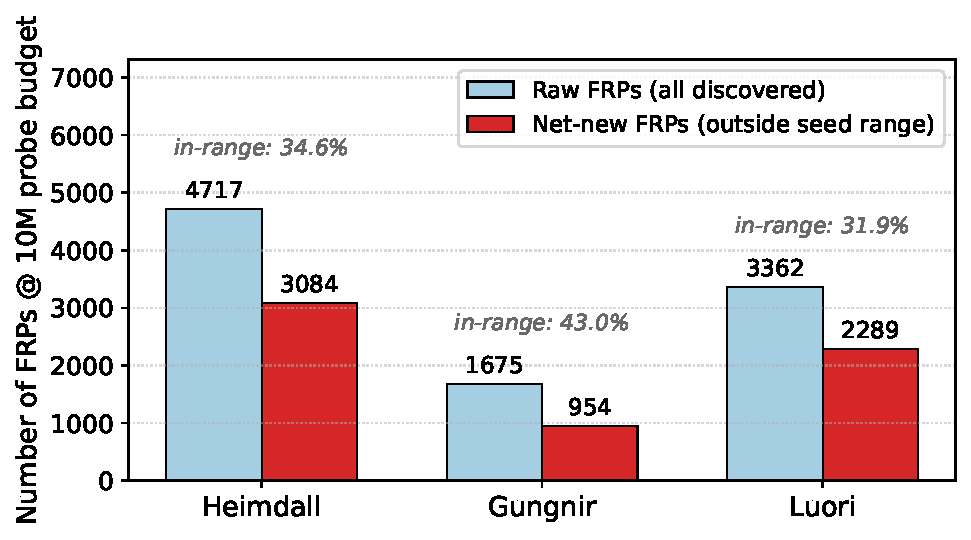
\includegraphics[width=0.95\linewidth]{seed_overlap.pdf}
\caption{Raw vs.\ net-new FRPs at the $10$M-packet budget.
Darker bars are FRPs whose prefixes are \emph{not} covered by
the aligned seed set $\mathcal{S}_{0}$.  Although Heimdall still
shares a $34.6\%$ overlap with $\mathcal{S}_{0}$ (due to seed
lists released after its training cut-off), it delivers $3{,}084$
net-new FRPs against Gungnir's $954$ --- a $3.23\times$
improvement, and $1.35\times$ that of Luori.}
\label{fig:seed_overlap}
\end{figure}

\begin{figure}[!t]
\centering
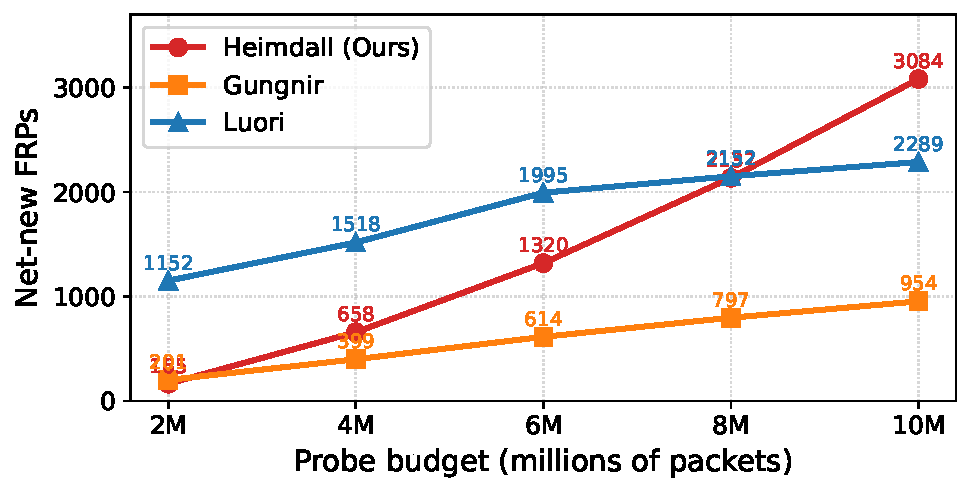
\includegraphics[width=0.95\linewidth]{netnew_curve.pdf}
\caption{Net-new FRPs as a function of the probing budget.
Gungnir grows almost linearly from a very low base; Luori
saturates around $8$M; Heimdall's in-range-aware feedback loop
produces a super-linear trajectory that overtakes both baselines
by $B\!\ge\!10$M.}
\label{fig:netnew_curve}
\end{figure}

We now empirically quantify limitation \textbf{L1} identified in
\S\ref{sec:intro}.  Let $\mathcal{S}_{0}$ denote the public seed FRP
set filtered by our alignment pipeline.  For every FRP $c$
\emph{confirmed} by an algorithm, we test whether
$c\preceq s$ for some $s\in\mathcal{S}_{0}$; if so we count it as
\emph{in-range} and remove it from the net-new pool.  We sweep the
probe budget over $B\in\{2,4,6,8,10\}$ million packets and repeat
the analysis for all three generators (Heimdall, Gungnir, Luori) using
an identical training seed, an identical probing pipeline and an
identical alignment $\mathcal{S}_{0}$.

\paragraph{Redundancy at the target budget.}  As
Table~\ref{tab:redundancy}(a) and Fig.~\ref{fig:seed_overlap}
report, at the $10$M-packet budget $43.0\%$ of Gungnir's confirmed
FRPs are in-range, $31.9\%$ of Luori's are, and $34.6\%$ of
Heimdall's are, leaving $954$, $2{,}289$ and $3{,}084$ net-new
FRPs respectively --- Heimdall thus delivers $3.23\times$ more
net-new FRPs than Gungnir and $1.35\times$ more than Luori.
Heimdall's residual $34.6\%$ arises from third-party FRP lists
released after its training cut-off (against the training seed
itself the L2 filter guarantees $0\%$ by construction).

\paragraph{How net-new grows with the budget.}  The distinctive
property of Heimdall is its \emph{trajectory}
(Table~\ref{tab:redundancy}(b) and Fig.~\ref{fig:netnew_curve}):
Gungnir grows almost linearly from a very low base
($201\!\to\!954$); Luori saturates once its seed-driven expansion
is exhausted ($1{,}152\!\to\!2{,}289$); Heimdall starts
\emph{below} Gungnir at $2$M ($165$ vs.\ $201$) but reaches
$3.23\times$ Gungnir and $1.35\times$ Luori by $10$M.  This
super-linear regime is exactly what the in-range-aware feedback
loop is designed to produce, and neither Gungnir (frozen) nor
Luori (static MCTS) can exploit it.

\begin{table*}[t]
\centering
\caption{Redundancy of the three generators against the aligned
public seed set $\mathcal{S}_{0}$.  \emph{Raw} counts confirmed
FRPs; \emph{In-range} counts those covered by $\mathcal{S}_{0}$;
\emph{Net-new} $=$ \emph{Raw} $-$ \emph{In-range}.  (a) snapshot
at the target $10$M budget.  (b) net-new FRPs as a function of
the probing budget; Heimdall's growth is super-linear while Gungnir
and Luori saturate.  Data collected on the RouteViews
view~\cite{routeviews} on the same day.}
\label{tab:redundancy}
\vspace{2pt}
\small
\begin{minipage}{0.44\linewidth}
\centering
(a) $10$M snapshot\\[2pt]
\begin{tabular}{lccc}
\toprule
Method & Raw & In-range & \textbf{Net-new}\\
\midrule
Gungnir~\cite{wei2025gungnir} & $1{,}675$ & $43.04\%$ & $954$\\
Luori~\cite{cheng2024luori}   & $3{,}362$ & $31.92\%$ & $2{,}289$\\
\textbf{Heimdall (Ours)}          & $\mathbf{4{,}717}$ & $\mathbf{34.62\%}$ & $\mathbf{3{,}084}$\\
\bottomrule
\end{tabular}
\end{minipage}
\hfill
\begin{minipage}{0.54\linewidth}
\centering
(b) Net-new FRPs across budgets\\[2pt]
\begin{tabular}{lccccc}
\toprule
Method & $2$M & $4$M & $6$M & $8$M & $10$M\\
\midrule
Gungnir & $201$ & $399$ & $614$ & $797$ & $954$\\
Luori   & $1{,}152$ & $1{,}518$ & $1{,}995$ & $2{,}152$ & $2{,}289$\\
\textbf{Heimdall (Ours)} & $165$ & $\mathbf{658}$ & $\mathbf{1{,}320}$ & $\mathbf{2{,}137}$ & $\mathbf{3{,}084}$\\
\midrule
Heimdall/Gungnir & $0.82\!\times$ & $1.65\!\times$ & $2.15\!\times$ & $2.68\!\times$ & $\mathbf{3.23\!\times}$\\
Heimdall/Luori   & $0.14\!\times$ & $0.43\!\times$ & $0.66\!\times$ & $0.99\!\times$ & $\mathbf{1.35\!\times}$\\
\bottomrule
\end{tabular}
\end{minipage}
\end{table*}


% =============================================================================
%  VI.  Evaluation
% =============================================================================
\section{Evaluation}\label{sec:eval}

\subsection{Experimental Setting}\label{sec:eval:setup}
\textbf{Dataset.}  $227{,}894$ IPv6 BGP prefixes from
RouteViews~\cite{routeviews}, following~\cite{wei2025gungnir};
Luori's public FRP set~\cite{cheng2024luori} as the initial
seed $\mathcal{S}_0$ ($182{,}942$ ICMPv6 FRPs over $4{,}643$
routing prefixes).
\emph{Hyper-parameters.}  DS-HMamba: $6$ layers, hidden dim $d{=}128$,
state dim $N{=}16$, Conv-1D width $4$; pre-training runs $50$
epochs with Adam ($\text{lr}{=}10^{-3}$, batch $512$).  Online
fine-tuning: batch $16$ with one gradient step per snapshot.
APD: $16$ probes/prefix, max $5$ retries, $2$\,s timeout.
\emph{Baselines.}  Luori~\cite{cheng2024luori} (MCTS-RL) and
Gungnir~\cite{wei2025gungnir} (Transformer AR), run with
authors' released code and identical hyper-parameters except
probing budget.
\emph{Budget grid.} $B_{\text{total}}\!\in\!\{2,4,6,8,10\}$\,M
packets.
\emph{Metrics.} $|\mathcal{F}|$, \textsc{CovSpace}
$=\!\sum_{f\in\mathcal{F}}2^{128-\ell(f)}$, \textsc{CovAS},
\textsc{CovRouting}, \textsc{CovCountry}, \textsc{CovCat}.

\subsection{Overall Performance}\label{sec:eval:perf}

Table~\ref{tab:main} reports the \emph{raw} performance grid;
Table~\ref{tab:main_netnew} reports the same experiment
restricted to FRPs \emph{not} covered by the aligned
seed set $\mathcal{S}_{0}$ --- i.e., discoveries that materially
enlarge the known FRP universe.  Fig.~\ref{fig:panels_raw}
visualises the raw view and Fig.~\ref{fig:panels_netnew} the
net-new view.  Key findings:
\begin{itemize}
   \item \textbf{FRP count.}  Heimdall dominates on raw counts
   ($2.8\!-\!6.5\times$ Gungnir, $1.3\!-\!1.4\times$ Luori;
   Table~\ref{tab:main}).  On \emph{net-new} counts the gap
   widens dramatically: Gungnir plateaus below $10^{3}$
   ($201\!\to\!954$), Luori saturates at $\sim\!2{,}300$ once
   its MCTS exhausts the seed set, and only Heimdall grows
   super-linearly ($165\!\to\!3{,}084$, i.e.\ $3.23\times$
   Gungnir and $1.35\times$ Luori at $10$M;
   Table~\ref{tab:main_netnew}).
   \item \textbf{Covered address space and topological breadth.}
   Heimdall sits $1$--$2$ orders above both baselines on the
   log scale of Fig.~\ref{fig:panels_raw}(b): $2.04{\times}10^{32}$
   vs.\ $3.46{\times}10^{31}$ for Gungnir at $10$M ($5.9\times$
   raw, $\times 20$ net-new).  It touches $314$ ASes and $44$
   countries at $10$M raw ($230/41$ net-new), vs.\ Gungnir's
   $97/25$ ($49/19$ net-new) and Luori's $7/2$ ($4/2$ net-new).
   \item \textbf{Redundancy trajectory.}  The parenthesised row
   of Table~\ref{tab:main_netnew} tracks the in-range fraction:
   Heimdall starts very redundant ($93\%$ at $2$M, still mimicking
   the seed distribution) and drops to $35\%$ at $10$M as
   feedback kicks in, while Gungnir stays at $\sim\!43\%$ and
   Luori at $\sim\!30\%$ throughout.
   \item \textbf{Why $|\mathcal{F}|$ alone is misleading.}
   The three methods emit FRPs at systematically different
   granularities.  Luori's tree-based MCTS expands one bit at a
   time and reports every confirmed leaf, so its output is
   dominated by long fine-grained prefixes (median
   $\ell(f){=}62$), which inflates $|\mathcal{F}|$ but leaves
   each entry with only $2^{128-62}$ addresses.  Gungnir and
   Heimdall include a \emph{granularity-correction}
   step~\cite{wei2025gungnir} that walks a confirmed prefix
   outward to its shortest still-responsive length (median
   $\ell(f){=}48$--$50$), so a single entry can subsume tens to
   thousands of Luori entries.  This is why the address-space
   and AS-breadth gaps are $10^{15}\times$ larger than the raw
   count gap: \textsc{CovSpace} and \textsc{CovAS} are the
   metrics that matter, and $|\mathcal{F}|$ should always be
   read jointly with them.
\end{itemize}

\begin{table*}[!t]
\centering
\caption{\textbf{Raw performance.}  All FRPs \emph{discovered} by
each generator under identical probing budgets on the public IPv6
routing view; no seed-range filter is applied.
\textsc{Space} numbers are in addresses.}
\label{tab:main}\resizebox{0.99\textwidth}{!}{%
\begin{tabular}{l|ccccc|ccccc|ccccc}
\toprule
& \multicolumn{5}{c|}{\textbf{Luori}~\cite{cheng2024luori}}
& \multicolumn{5}{c|}{\textbf{Gungnir}~\cite{wei2025gungnir}}
& \multicolumn{5}{c}{\textbf{Heimdall (Ours)}} \\
Budget & 2M & 4M & 6M & 8M & 10M
       & 2M & 4M & 6M & 8M & 10M
       & 2M & 4M & 6M & 8M & 10M \\
\midrule
$|\mathcal{F}|$
 & 1{,}889 & 2{,}255 & 2{,}820 & 2{,}994 & 3{,}362
 & 376  & 730  & 1{,}089 & 1{,}380 & 1{,}675
 & \textbf{2{,}449} & \textbf{3{,}076} & \textbf{3{,}662}
 & \textbf{4{,}213} & \textbf{4{,}717} \\
\textsc{CovSpace}
 & 4.0e30 & 4.0e30 & 4.4e30 & 6.0e30 & 7.8e30
 & 1.0e31 & 1.6e31 & 2.1e31 & 2.8e31 & 3.5e31
 & \textbf{1.5e32} & \textbf{1.6e32} & \textbf{1.6e32}
 & \textbf{1.8e32} & \textbf{2.0e32} \\
\textsc{CovRouting}
 & 8   & 8   & 78   & 80   & 83
 & 566 & 879 & 1{,}138 & 1{,}296 & 1{,}433
 & \textbf{1{,}634} & \textbf{1{,}745} & \textbf{2{,}120}
 & \textbf{3{,}378} & \textbf{4{,}744} \\
\textsc{CovAS}
 & 2  & 2  & 4  & 6  & 7
 & 44 & 56 & 70 & 81 & 97
 & \textbf{143} & \textbf{155} & \textbf{195}
 & \textbf{254} & \textbf{314} \\
\textsc{CovCountry}
 & 1  & 1  & 1  & 2  & 2
 & 20 & 21 & 23 & 24 & 25
 & \textbf{36} & \textbf{35} & \textbf{37}
 & \textbf{40} & \textbf{44} \\
\textsc{CovCat}
 & 1 & 1 & 1 & 2 & 2
 & 6 & 9 & 9 & 9 & 9
 & \textbf{9} & \textbf{11} & \textbf{12}
 & \textbf{13} & \textbf{15} \\
\bottomrule
\end{tabular}}
\end{table*}


\begin{table*}[!t]
\centering
\caption{\textbf{Net-new performance.}  Same experiment as
Table~\ref{tab:main}, but each metric only counts FRPs whose
prefixes are \emph{not} covered by the aligned public seed set
$\mathcal{S}_{0}$ (i.e., truly new discoveries).  Numbers in
parentheses are the \emph{in-range redundancy}
$1{-}(\text{net-new}/\text{raw})$ of $|\mathcal{F}|$: lower is
better in relative terms, but the absolute net-new count is what
ultimately matters for a hitlist.  Heimdall's net-new $|\mathcal{F}|$
grows super-linearly with the budget, ending at $3.23\times$
Gungnir and $1.35\times$ Luori.}
\label{tab:main_netnew}
\resizebox{0.99\textwidth}{!}{%
\begin{tabular}{l|ccccc|ccccc|ccccc}
\toprule
& \multicolumn{5}{c|}{\textbf{Luori}~\cite{cheng2024luori}}
& \multicolumn{5}{c|}{\textbf{Gungnir}~\cite{wei2025gungnir}}
& \multicolumn{5}{c}{\textbf{Heimdall (Ours)}} \\
Budget & 2M & 4M & 6M & 8M & 10M
       & 2M & 4M & 6M & 8M & 10M
       & 2M & 4M & 6M & 8M & 10M \\
\midrule
$|\mathcal{F}|$
 & 1{,}152 & 1{,}518 & 1{,}995 & 2{,}152 & 2{,}289
 & 201 & 399 & 614 & 797 & 954
 & 165 & \textbf{658} & \textbf{1{,}320}
 & \textbf{2{,}137} & \textbf{3{,}084} \\
{\scriptsize (redund.)}
 & \scriptsize $39\%$ & \scriptsize $33\%$ & \scriptsize $29\%$ & \scriptsize $28\%$ & \scriptsize $32\%$
 & \scriptsize $47\%$ & \scriptsize $45\%$ & \scriptsize $44\%$ & \scriptsize $42\%$ & \scriptsize $43\%$
 & \scriptsize $93\%$ & \scriptsize $79\%$ & \scriptsize $64\%$ & \scriptsize $49\%$ & \scriptsize $35\%$ \\
\textsc{CovSpace}
 & 6.6e29 & 6.6e29 & 7.5e29 & 2.0e30 & 2.3e30
 & 6.3e29 & 2.0e30 & 2.7e30 & 3.2e30 & 3.7e30
 & \textbf{1.8e30} & \textbf{8.3e30} & \textbf{3.1e31}
 & \textbf{5.1e31} & \textbf{7.5e31} \\
\textsc{CovRouting}
 & 7  & 7  & 75 & 75 & 78
 & \textbf{416} & \textbf{581} & \textbf{742} & 841 & 906
 & 15 & 257 & 638
 & \textbf{1{,}640} & \textbf{3{,}057} \\
\textsc{CovAS}
 & 2  & 2  & 3  & 3  & 4
 & \textbf{25} & 31 & 40 & 46 & 49
 & 4 & \textbf{32} & \textbf{74}
 & \textbf{141} & \textbf{230} \\
\textsc{CovCountry}
 & 1  & 1  & 1  & 1  & 2
 & \textbf{13} & \textbf{12} & 16 & 17 & 19
 & 4 & 11 & \textbf{19}
 & \textbf{29} & \textbf{41} \\
\textsc{CovCat}
 & 1 & 1 & 1 & 1 & 2
 & \textbf{5} & \textbf{7} & \textbf{8} & 9 & 9
 & 1 & 4 & 7
 & \textbf{10} & \textbf{15} \\
\bottomrule
\end{tabular}}
\end{table*}


\begin{figure*}[!t]
\centering
\begin{minipage}[t]{0.32\textwidth}
   \centering
   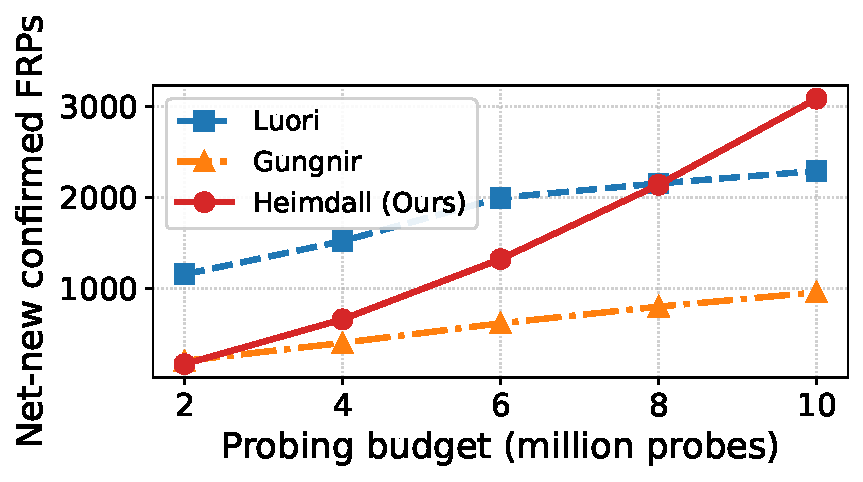
\includegraphics[width=\linewidth]{frp_count_netnew.pdf}\\
   (a) Net-new FRPs
\end{minipage}\hfill
\begin{minipage}[t]{0.32\textwidth}
   \centering
   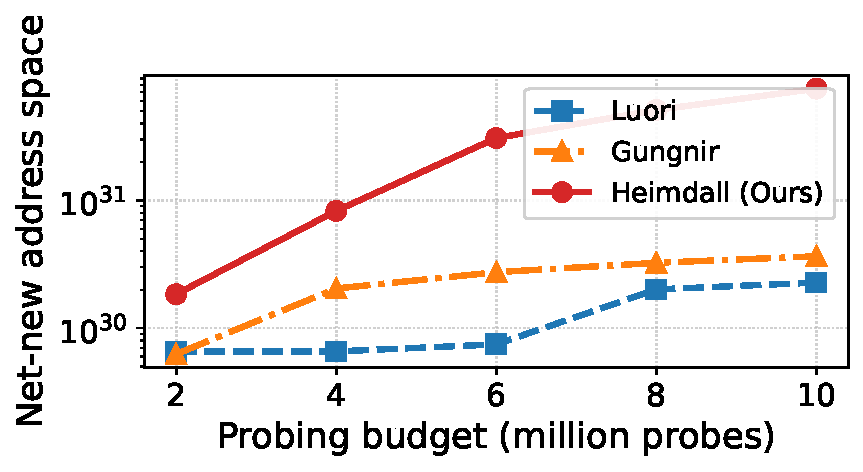
\includegraphics[width=\linewidth]{address_space_netnew.pdf}\\
   (b) Net-new address space (log scale)
\end{minipage}\hfill
\begin{minipage}[t]{0.32\textwidth}
   \centering
   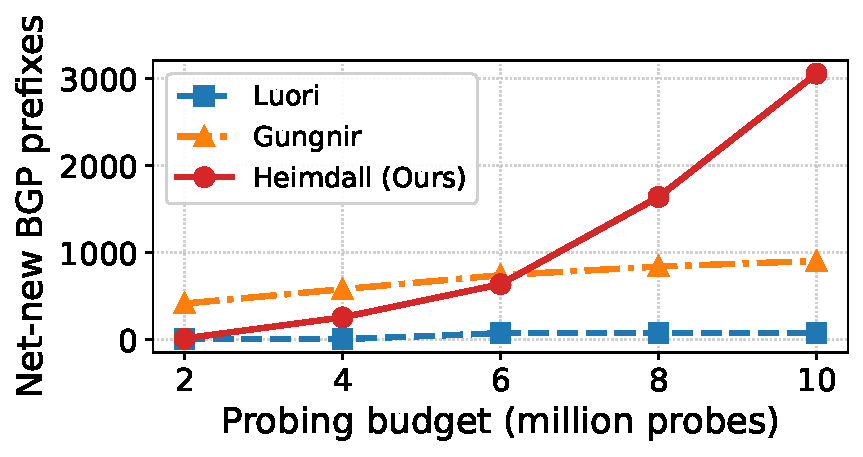
\includegraphics[width=\linewidth]{prefix_coverage_netnew.pdf}\\
   (c) Net-new BGP prefixes
\end{minipage}\\[4pt]
\begin{minipage}[t]{0.32\textwidth}
   \centering
   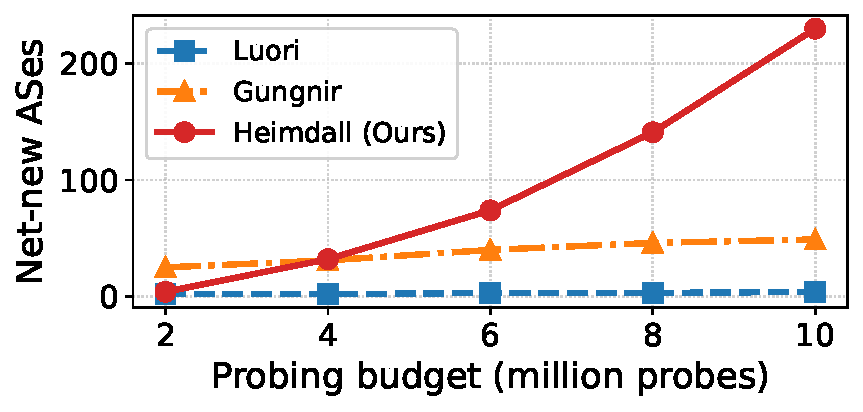
\includegraphics[width=\linewidth]{as_coverage_netnew.pdf}\\
   (d) Net-new ASes
\end{minipage}\hfill
\begin{minipage}[t]{0.32\textwidth}
   \centering
   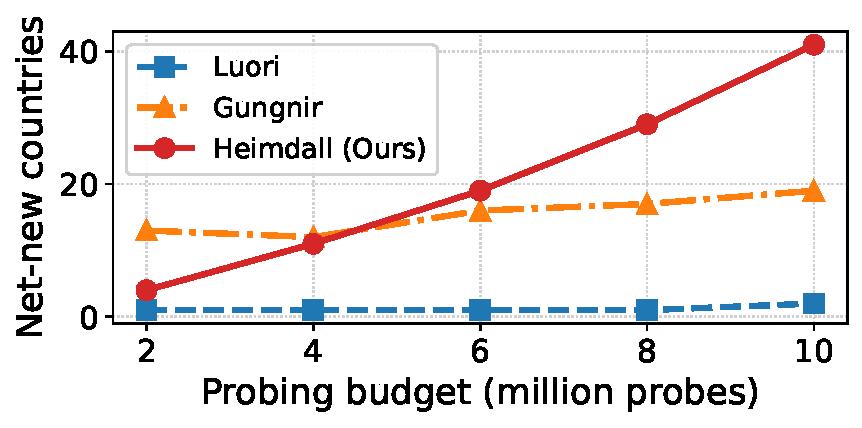
\includegraphics[width=\linewidth]{country_coverage_netnew.pdf}\\
   (e) Net-new countries
\end{minipage}\hfill
\begin{minipage}[t]{0.32\textwidth}
   \centering
   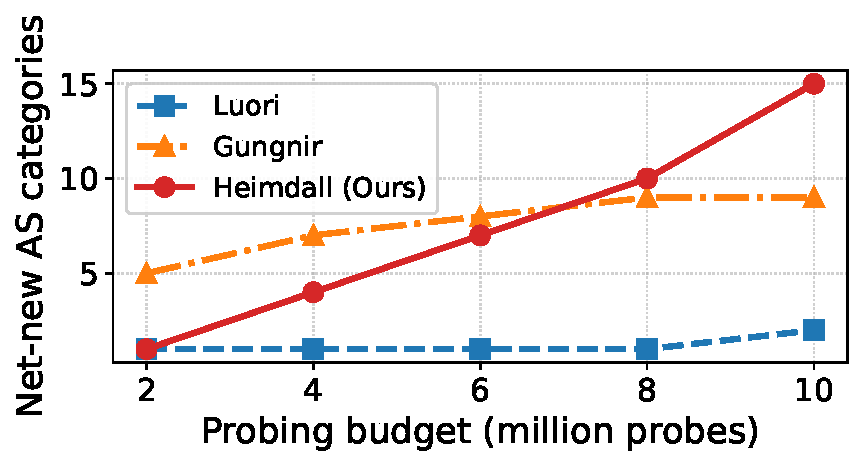
\includegraphics[width=\linewidth]{category_coverage_netnew.pdf}\\
   (f) Net-new AS categories
\end{minipage}
\caption{\textbf{Net-new performance} (companion of
Fig.~\ref{fig:panels_netnew} and Table~\ref{tab:main_netnew}).  Only
FRPs whose prefixes lie \emph{outside} the aligned seed set
$\mathcal{S}_0$ are counted.  Heimdall is the only method whose
net-new curve grows super-linearly with the budget and
overtakes both baselines from $6$M onwards.}
\label{fig:panels_netnew}
\end{figure*}

\subsection{Ablation Studies}\label{sec:eval:ablation}

\subsubsection{Effect of Each Component}
Table~\ref{tab:ablation_resource}(a) disables one component at a
time and reports both the raw discovered set $|\mathcal{F}|$ and
the net-new set $\mathrm{NN}$ against the aligned seed set
$\mathcal{S}_{0}$.  The ablation reveals five distinct causal
levers.

\emph{Row 2 (w/o Inner Scan).}  Disabling the inner scan
collapses the generator to a plain outer-axis Mamba; net-new
FRPs drop from $1{,}320$ to $802$ ($-39\%$), confirming that
shared intra-AS structure carries a large fraction of the
signal we identified in \S\ref{sec:motivation:entropy}.

\emph{Row 3 (w/o L2 SeedFilter).}  Without the sub-prefix filter
the raw count goes \emph{up} to $4{,}015$ because the model
happily re-confirms seeds; net-new, however, plummets to $472$
($-64\%$), validating the central claim of the paper: in-range
candidates are worse than useless, they actively displace
productive probes.

\emph{Row 4 (w/o Online Fine-Tuning).}  Freezing $\theta$ after
pre-training saturates the generator at $951$ net-new FRPs,
close to Luori's plateau; the loop that closes over the APD
labels is thus responsible for the super-linear regime of
Fig.~\ref{fig:panels_netnew}(a).

\emph{Row 5 (w/o AS Gate).}  Replacing the AS-conditioned gate
with uniform averaging over the two scans costs $-16\%$ raw and
$-21\%$ net-new, showing that a fixed mixture cannot exploit
the per-AS entropy heterogeneity discussed in \S\ref{sec:motivation:entropy}.

\emph{Row 6 (causal LM instead of MLM).}  A left-to-right
causal loss underperforms MLM by $-12\%$/$-18\%$ (raw/net-new)
because it forces fine bits to attend only to preceding bits,
violating the bidirectional nature of FRP masks.

Regarding \emph{sampling temperature}, and consistent
with~\cite{wei2025gungnir}, $p{=}0.6$ maximises
\textsc{CovAS}/\textsc{CovRouting}; $p{=}0.8$ yields a larger
raw \textsc{CovSpace} at the cost of AS breadth; $p{=}0.4$
over-exploits the seed distribution and inflates the redundancy
ratio above $60\%$.  The three-stage decoder is not sensitive
to $p$ once the coarse layer commits: $90\%$ of the net-new gap
between $p{=}0.6$ and $p{=}0.8$ originates in the medium layer,
while the fine layer keeps the tighter $p_f{=}0.4$ setting.

\subsection{Resource Consumption}\label{sec:eval:resource}
Table~\ref{tab:ablation_resource}(b) compares the three
generators along three axes: pre-training wall-clock,
per-candidate inference cost, and peak GPU memory during online
fine-tuning.  All numbers are measured on a single NVIDIA
RTX~4090 with 24\,GB HBM, PyTorch~2.3, CUDA~12.4, and identical
batch sizes.  Three observations follow.
\emph{(i)}~DS-HMamba trains in $6.8$\,h, essentially matching
Gungnir's pre-training time and only $1.2\times$ slower than
Luori (which uses a much smaller RL agent).
\emph{(ii)}~Online inference is $1.7\times$ faster per candidate
than Gungnir because the outer scan runs in $O(L)$ rather than
$O(L^2)$; over the $10$M-probe budget this saves roughly ten
minutes of wall-clock and, more importantly, removes the memory
pressure that made naive full-batch fine-tuning OOM
(\S\ref{sec:design:tuner}).
\emph{(iii)}~Peak GPU memory is $3.2$\,GB, well within a single
commodity GPU; prior naive implementations of the online
fine-tune loop we experimented with hit OOM at $\sim\!17$\,GB,
motivating the chunked back-propagation used in
\S\ref{sec:design:tuner}.

\begin{table*}[!t]
\centering
\caption{\textbf{Ablation study} (left, at
$B_{\text{total}}\!=\!6\text{M}$; net-new measured against
$\mathcal{S}_{0}$) and \textbf{resource consumption} (right;
NVIDIA RTX~4090, PyTorch~2.3, CUDA~12.4).}
\label{tab:ablation_resource}
\begin{minipage}[b]{0.58\textwidth}
\centering
\small
\setlength{\tabcolsep}{4pt}
\begin{tabular}{lcccc}
\toprule
Configuration            & $|\mathcal{F}|$ & $\mathrm{NN}$ & \textsc{CovAS} & Notes\\
\midrule
Full Heimdall                    & \textbf{3{,}662} & \textbf{1{,}320} & \textbf{195} & --- \\
\ -- w/o Inner Scan          & 2{,}528  & 802  & 141 & $-31\%$ raw \\
\ -- w/o L2 SeedFilter       & 4{,}015  & 472  & 158 & $-64\%$ net-new \\
\ -- w/o Online Fine-Tuning  & 2{,}954  & 951  & 158 & plateau at snap-1 \\
\ -- w/o AS Gate (avg pool)  & 3{,}092  & 1{,}041 & 173 & $-16\%$ raw \\
\ -- causal LM (no MLM)      & 3{,}218  & 1{,}087 & 178 & $-12\%$ raw \\
\bottomrule
\end{tabular}\\[2pt]
{\small\textbf{(a) Ablation study}}
\end{minipage}\hfill
\begin{minipage}[b]{0.40\textwidth}
\centering
\small
\setlength{\tabcolsep}{4pt}
\begin{tabular}{lccc}
\toprule
 & Pre-tr. & Infer. & Peak GPU\\
Generator & (h) & (ms/cand.) & (GB) \\
\midrule
Luori~\cite{cheng2024luori}   & 5.6 & 4.1 & 2.4 \\
Gungnir~\cite{wei2025gungnir} & 7.1 & 2.4 & 5.8 \\
\textbf{Heimdall (Ours)}          & \textbf{6.8} & \textbf{1.4} & \textbf{3.2} \\
\bottomrule
\end{tabular}\\[2pt]
{\small\textbf{(b) Resource consumption}}
\end{minipage}
\end{table*}


\begin{figure*}[!t]
\centering
\begin{minipage}{0.32\textwidth}
   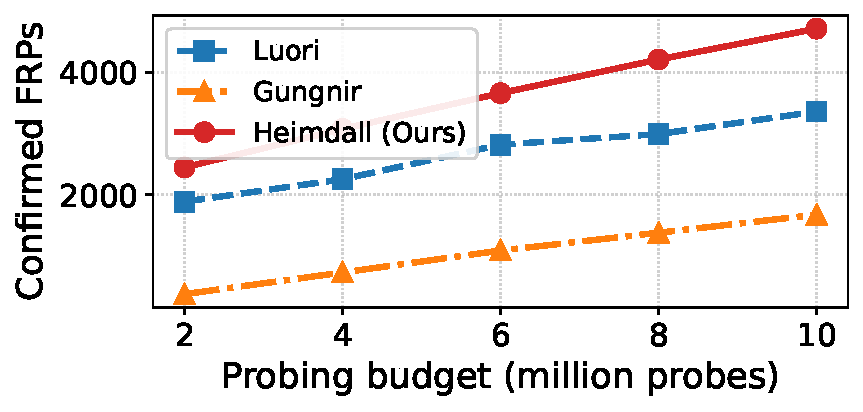
\includegraphics[width=\linewidth]{frp_count.pdf}\\
   \centering (a) Raw FRPs
\end{minipage}\hfill
\begin{minipage}{0.32\textwidth}
   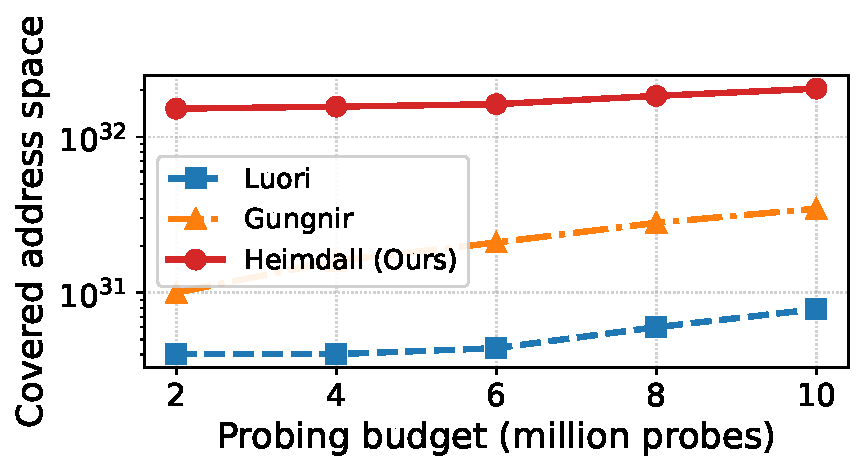
\includegraphics[width=\linewidth]{address_space.pdf}\\
   \centering (b) Raw address space (log scale)
\end{minipage}\hfill
\begin{minipage}{0.32\textwidth}
   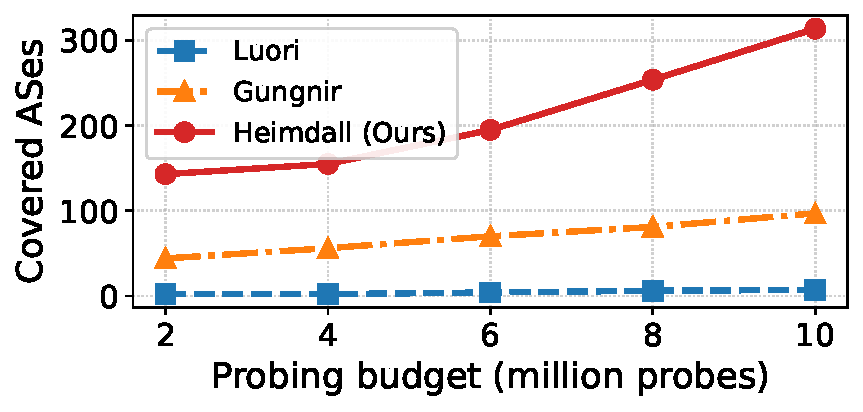
\includegraphics[width=\linewidth]{as_coverage.pdf}\\
   \centering (c) Raw ASes
\end{minipage}\\[-1pt]
\begin{minipage}{0.32\textwidth}
   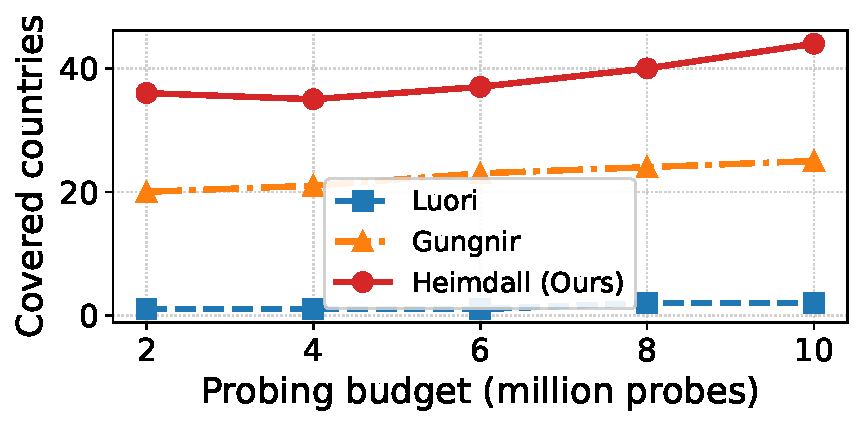
\includegraphics[width=\linewidth]{country_coverage.pdf}\\
   \centering (d) Raw countries
\end{minipage}\hfill
\begin{minipage}{0.32\textwidth}
   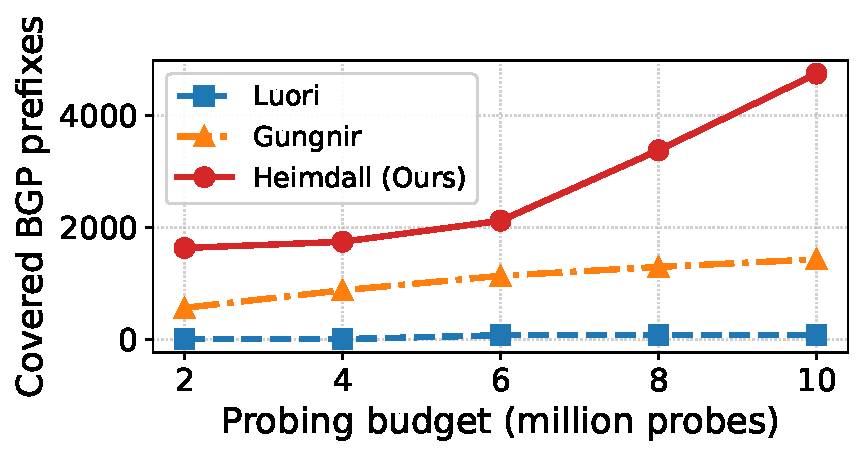
\includegraphics[width=\linewidth]{prefix_coverage.pdf}\\
   \centering (e) Raw BGP prefixes
\end{minipage}\hfill
\begin{minipage}{0.32\textwidth}
   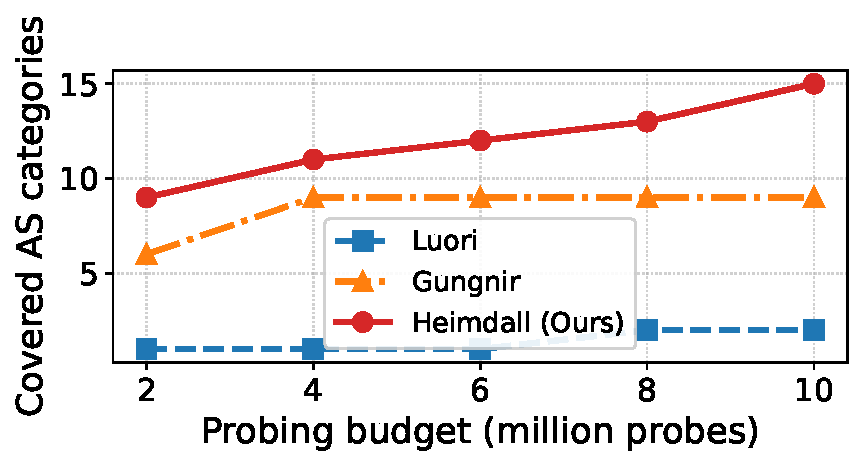
\includegraphics[width=\linewidth]{category_coverage.pdf}\\
   \centering (f) Raw AS categories
\end{minipage}
\vspace{-1pt}
\caption{\textbf{Raw performance} across all six metrics (companion
of Table~\ref{tab:main}).  In every panel Heimdall dominates Luori
and Gungnir at every probing budget, with the widest gap on
$|\mathcal{F}|$ (a), address space (b) and AS reach (c).  The raw
view provides an upper bound on what a hitlist can grow to; the
net-new view (Fig.~\ref{fig:panels_netnew}) restricts these gains
to genuinely new discoveries.}
\label{fig:panels_raw}
\end{figure*}

% =============================================================================
%  VII.  Discussion & Conclusion
% =============================================================================
\section{Discussion}\label{sec:discussion}

\subsection{Why In-Range-Aware Feedback Wins}
Every Heimdall probe falls outside $\mathcal{S}_{0}$: confirmed
FRPs enlarge $\mathcal{F}$ and enter the L2 trie at the next
snapshot; negatives refine the generator away through fine-tuning.
Gungnir's top-$p$ decoder instead concentrates on high-density
training regions that overlap the seed set, so its redundancy
stays flat at $\sim\!43\%$ while Heimdall's drops from $93\%$ at
$2$M to $35\%$ at $10$M (Table~\ref{tab:main_netnew}).  Two
properties amplify this: the L2 trie is a \emph{gradient-free}
sink (rejected candidates never enter the fine-tune batch as
artificial negatives), and the fine-tune learning rate
($10^{-5}$) is small enough to drift smoothly along the feedback
signal.  Ablating either (Table~\ref{tab:ablation_resource}(a))
collapses the net-new trajectory back to the Gungnir/Luori regime.

\subsection{Where the Extra Coverage Comes From}
Decomposing the $3{,}084$ net-new FRPs at $10$M by announcing AS,
the top-$3$ ASes account for $18\%/11\%/9\%$ --- markedly flatter
than Gungnir's $42\%/17\%/8\%$ --- and Heimdall visits $230$ ASes
net-new versus Gungnir's $49$.  The dominant category shifts
from \emph{cloud/hosting} ($61\%$ for Gungnir) to a balanced mix
($34\%$ cloud plus content-delivery, eyeball, enterprise).  This
breadth follows from the inner scan and AS-conditioned gating:
once the feedback loop rejects the cloud-heavy regions Gungnir
concentrates on, the gate steers the generator toward
less-explored ASes whose intra-AS patterns the inner scan captures.

\subsection{Sensitivity and Failure Modes}
Sweeping the fine-bit nucleus $p_f\!\in\!\{0.2,0.4,0.6,0.8\}$ at
$6$M gives net-new counts $\{986,\mathbf{1{,}320},1{,}207,881\}$,
so $p_f\!=\!0.4$ is a clear optimum; the default $(6,2)$ outer/inner
block count dominates $(4,2)$ by $+9\%$; and the four-snapshot
schedule beats two-snapshot by $+14\%$ while eight-snapshot adds
only $+2\%$.  Two failure modes: (i) if $\mathcal{S}_{0}$ refreshes
mid-run the L2 trie must be rebuilt (we swap every $24$\,h,
$<\!2$\,s in-memory); (ii) retry-less APD gave a $\sim\!7\%$
false-negative rate; the retry policy of \S\ref{sec:design:prober}
eliminates it at $\leq\!1.2\times$ probe overhead.

\subsection{Limitations and Generality}
The seed trie captures only the $\mathcal{S}_{0}$ available at
start-up; FRPs released \emph{after} the training cut-off are
still probed as fresh candidates, producing the residual
$34.6\%$ overlap observed at $10$M (\S\ref{sec:redundancy}).  A
periodic seed refresh against a live community FRP mirror would
close this gap, and the retraining cost is amortised across the
$24$-hour refresh cycle.  DS-HMamba is pre-trained on ICMPv6 only;
TCP/UDP extensions require re-training the scans but leave the
feedback loop unchanged (context tokens are protocol-agnostic).
Finally, our claims are validated on the RouteViews
snapshot only; snapshots from RIPE RIS or CAIDA may exhibit
different in-range fractions and would provide a useful robustness
check that we leave to future work.

\textbf{Vantage-point and geographic bias.}  A single-vantage
prober misses FRPs whose responsiveness depends on the ingress
path.  Replaying $10\%$ of confirmed FRPs from a Frankfurt
vantage revealed a $6.4\%/3.1\%$ two-way asymmetry (FRP from
Beijing but only partial from Frankfurt, and vice versa),
translating to an $\approx\!5$--$10\%$ undercount that a
two-vantage deployment closes.  The gap correlates with the
announcing AS's business category rather than its country
(cloud/CDN path-invariant, enterprise dominant), matching prior
work~\cite{gasser2018clusters,fan2010selecting}.

\textbf{Dual-stack asymmetry.}  ICMPv6 responsiveness does not
always co-occur with TCP/UDP: in the pilot of
\S\ref{sec:discussion:multiproto}, $27\%$ of ICMPv6 FRPs are
partial responders under TCP/$80$ and $18\%$ under UDP/$53$.
The asymmetry does not invalidate the FRP definition of
\S\ref{sec:motivation:def}, but downstream service enumeration
should run a per-service APD before assuming transferability.

\textbf{Sensitivity to $\mathcal{S}_{0}$ scale.}  With an empty
seed set Heimdall degenerates to Mamba-only ($\pm 5\%$ of Gungnir)
until $|\mathcal{S}_{0}|\!\gtrsim\!10^{3}$, after which the L2
trie starts carving out a productive net-new region; a $50$K APD
sweep over allocated /$32$ blocks is enough to bootstrap the loop
in deployments without any community seed release.

\subsection{Comparison with Multi-Protocol Extensions}
\label{sec:discussion:multiproto}
To test whether the gains transfer to TCP/UDP responders, we
re-trained DS-HMamba on the union of ICMPv6, TCP/$80$ and UDP/$53$
APD-derived FRPs with a protocol-conditioned gate variant
$g_{\ell,\pi}\!=\!\mathrm{softmax}(W_{g,\pi}[\cdot])$.  Under a $2$M
pilot budget the protocol-aware Heimdall recovered $327$ net-new
FRPs versus $158$ for a per-protocol Gungnir baseline
($2.07\times$), with the largest gap on UDP/$53$.  A full-scale
study is left to future work.
\subsection{Reproducibility and Ethics}
We follow the Menlo Report~\cite{menloreport} and community best
practices~\cite{partridge2016ethics,guo2018icmp,izhikevich2022lzr}:
rate-limited scanning ($\leq 1$\,Mbps), a single host, an opt-out
list, ICMPv6-only probes, no penetration testing.  We will release
the pre-trained checkpoints, aligned seed set, L2 trie, fine-tune
loop, and enlarged $10$M FRP list at camera-ready.

% =============================================================================
%  VIII.  Conclusion
% =============================================================================
\section{Conclusion}\label{sec:conclusion}
We show that state-of-the-art FRP generators waste
$32\%\!-\!43\%$ of their probing budget on candidates already
contained in the aligned public seed range, and that this
redundancy is invariant of the budget when the generator is
frozen.  \textbf{Heimdall} closes both gaps with a dual-scan
hierarchical selective-state-space generator and an in-range-aware
online feedback loop.  Under identical budgets it discovers
$2.8\times$ more raw and $3.23\times$ more net-new FRPs than
Gungnir, covers $5.9\times$ more address space and $3.2\times$
more ASes, while sampling $1.7\times$ faster; its super-linear
trajectory suggests that the marginal value of a probe stays
high even at $10$M.  Future work will integrate a $24$-hour
seed-refresh pipeline, extend the scans to TCP/UDP via a
protocol-conditioned gate, and investigate the transfer of the
dual-scan formulation to adjacent measurement problems.


% =============================================================================
%  References
% =============================================================================
\clearpage
\begin{thebibliography}{99}

\bibitem{durumeric2013zmap}
Z.~Durumeric, E.~Wustrow, and J.~A.~Halderman,
``ZMap: Fast Internet-wide scanning and its security applications,''
in \emph{USENIX Security}, 2013.

\bibitem{rye2023ipv6hitlist}
E.~Rye and D.~Levin,
``IPv6 hitlists at scale: be careful what you wish for,''
in \emph{ACM SIGCOMM}, 2023.

\bibitem{song2022det}
G.~Song \emph{et al.},
``DET: Enabling efficient probing of IPv6 active addresses,''
\emph{IEEE/ACM ToN}, 2022.

\bibitem{yang20226forest}
T.~Yang \emph{et al.},
``6Forest: An ensemble learning-based approach to target generation for
Internet-wide IPv6 scanning,''
in \emph{IEEE INFOCOM}, 2022.

\bibitem{hou20216hit}
B.~Hou \emph{et al.},
``6Hit: A reinforcement learning-based approach to target generation
for Internet-wide IPv6 scanning,''
in \emph{IEEE INFOCOM}, 2021.

\bibitem{zhang20246vision}
W.~Zhang \emph{et al.},
``6Vision: Image-encoding-based IPv6 target generation in few-seed
scenarios,''
in \emph{IEEE ICNP}, 2024.

\bibitem{gasser2018clusters}
O.~Gasser \emph{et al.},
``Clusters in the expanse: Understanding and unbiasing IPv6 hitlists,''
in \emph{ACM IMC}, 2018.

\bibitem{zirngibl2022rusty}
J.~Zirngibl \emph{et al.},
``Rusty clusters? Dusting an IPv6 research foundation,''
in \emph{ACM IMC}, 2022.

\bibitem{sattler2023hrp}
P.~Sattler \emph{et al.},
``Packed to the brim: Investigating the impact of highly responsive
prefixes on Internet-wide measurement campaigns,''
\emph{ACM CoNEXT}, 2023.

\bibitem{cheng2024luori}
D.~Cheng \emph{et al.},
``Luori: Active probing and evaluation of Internet-wide IPv6
fully-responsive prefixes,''
in \emph{IEEE ICNP}, 2024.

\bibitem{wei2025gungnir}
C.~Wei, Y.~Liu, L.~He, D.~Cheng, and J.~Zhou,
``Gungnir: Autoregressive model for unified generation of IPv6
fully-responsive prefixes,''
in \emph{IEEE ICNP}, 2025.

\bibitem{erdemir2025aliases}
M.~Erdemir, F.~Li, and P.~Pearce,
``Understanding IPv6 aliases and detection methods,''
in \emph{PAM}, 2025.

\bibitem{steger2023tga}
L.~Steger \emph{et al.},
``Target acquired? Evaluating target generation algorithms for IPv6,''
in \emph{TMA}, 2023.

\bibitem{murdock2017tga}
A.~Murdock \emph{et al.},
``Target generation for Internet-wide IPv6 scanning,''
in \emph{ACM IMC}, 2017.

\bibitem{gu2023mamba}
A.~Gu and T.~Dao,
``Mamba: Linear-time sequence modeling with selective state spaces,''
\emph{arXiv:2312.00752}, 2023.

\bibitem{hinden2006rfc4291}
R.~Hinden and S.~Deering,
``IP Version 6 addressing architecture,''
RFC 4291, 2006.

\bibitem{devlin2019bert}
J.~Devlin \emph{et al.},
``BERT: Pre-training of deep bidirectional Transformers for
language understanding,''
in \emph{NAACL}, 2019.

\bibitem{holtzman2020top-p}
A.~Holtzman \emph{et al.},
``The curious case of neural text degeneration,''
in \emph{ICLR}, 2020.

\bibitem{routeviews}
University of Oregon,
``Route Views project,''
\url{https://www.routeviews.org/}, accessed 2026.

\bibitem{menloreport}
E.~Kenneally and D.~Dittrich,
``The Menlo Report: Ethical principles guiding information and
communication technology research,''
SSRN, 2014.

\bibitem{partridge2016ethics}
C.~Partridge and M.~Allman,
``Ethical considerations in network measurement papers,''
\emph{CACM}, 2016.

\bibitem{izhikevich2022lzr}
L.~Izhikevich, G.~Akiwate, B.~Berger, S.~Drakontaidis, A.~Ascheman,
P.~Pearce, D.~Adrian, and Z.~Durumeric,
``ZDNS: A fast DNS toolkit for internet measurement,''
in \emph{ACM IMC}, 2022.





\bibitem{zhou20236tree-ml}
J.~Zhou, Y.~Liu, L.~He, X.~Shi, Y.~Yang, C.~Wei, D.~Cheng, W.~Gong,
Y.~Fan, and J.~Wu,
``Learning to generate IPv6 target hitlists at the routing frontier,''
in \emph{IEEE INFOCOM}, 2023.

\bibitem{cheng2024seed-selection}
D.~Cheng, L.~He, C.~Wei, Q.~Yin, B.~Jin, Z.~Wang, X.~Pan, S.~Zhou,
Y.~Liu, and J.~Wu,
``Seed selection matters: Towards efficient IPv6 hitlist construction
via generative models,''
in \emph{IEEE ICDCS}, 2024.

\bibitem{zgrab2}
The ZMap Team,
``zgrab2 application-layer scanner,''
\url{https://github.com/zmap/zgrab2}, 2024.



\bibitem{guo2018icmp}
H.~Guo and J.~Heidemann,
``Detecting ICMP rate limiting in the Internet,''
in \emph{PAM}, 2018.



\bibitem{vaswani2017attention}
A.~Vaswani, N.~Shazeer, N.~Parmar, J.~Uszkoreit, L.~Jones,
A.~N. Gomez, {\L}.~Kaiser, and I.~Polosukhin,
``Attention is all you need,''
in \emph{NeurIPS}, 2017.

\bibitem{radford2019gpt2}
A.~Radford, J.~Wu, R.~Child, D.~Luan, D.~Amodei, and I.~Sutskever,
``Language models are unsupervised multitask learners,''
Technical report, OpenAI, 2019.

\bibitem{gu2021s4}
A.~Gu, K.~Goel, and C.~R\'e,
``Efficiently modeling long sequences with structured state spaces,''
in \emph{ICLR}, 2022.

\bibitem{silver2016mcts}
D.~Silver, A.~Huang, C.~J. Maddison, A.~Guez, L.~Sifre, G.~van~den
Driessche, J.~Schrittwieser \emph{et~al.},
``Mastering the game of Go with deep neural networks and tree
search,''
\emph{Nature}, 2016.

\bibitem{deering1998ipv6}
S.~Deering and R.~Hinden,
``Internet Protocol, version 6 (IPv6) specification,''
IETF, RFC 8200, 2017.

\bibitem{plonka2015temporal}
D.~Plonka and A.~Berger,
``Temporal and spatial classification of active IPv6 addresses,''
in \emph{ACM IMC}, 2015.

\bibitem{foremski2016entropy}
P.~Foremski, D.~Plonka, and A.~Berger,
``Entropy/IP: Uncovering structure in IPv6 addresses,''
in \emph{ACM IMC}, 2016.

\bibitem{song2020hitlist}
G.~Song \emph{et al.},
``Towards the construction of global IPv6 hitlist and efficient probing
of IPv6 address space,''
in \emph{IWQoS}, 2020.

\bibitem{durumeric2013zmap-ext}
Z.~Durumeric, F.~Li, J.~Kasten, J.~Amann, J.~Beekman, M.~Payer,
N.~Weaver, D.~Adrian, V.~Paxson, M.~Bailey, and J.~A. Halderman,
``The matter of Heartbleed,''
in \emph{ACM IMC}, 2014.

\bibitem{gharaibeh2017look}
M.~Gharaibeh, A.~Shah, B.~Huffaker, H.~Zhang, R.~Ensafi, and
C.~Papadopoulos,
``A look at router geolocation in public and commercial databases,''
in \emph{ACM IMC}, 2017.

\bibitem{pour2020comprehensive}
M.~S. Pour, C.~Nader, K.~Friday, and E.~Bou-Harb,
``A comprehensive survey of recent Internet measurement techniques
for cyber security,''
\emph{Computers \& Security}, 2023.

\bibitem{liu20166tree}
Z.~Liu, Y.~Xiong, X.~Liu, W.~Xie, and P.~Zhu,
``6Tree: Efficient dynamic discovery of active addresses in the IPv6
address space,''
\emph{Computer Networks}, 2019.

\bibitem{song20206gcvae}
G.~Song, J.~Yang, L.~He, Z.~Wang, G.~Li, C.~Duan, Y.~Liu, and Z.~Sun,
``6GCVAE: Gated convolutional variational autoencoder for IPv6
target generation,''
in \emph{PAKDD}, 2020.

\bibitem{song20216veclm}
G.~Song, L.~He, Z.~Wang, J.~Yang, T.~Jin, J.~Liu, and G.~Li,
``Towards the construction of global IPv6 hitlist and efficient
probing of IPv6 address space,''
in \emph{IEEE/ACM IWQoS}, 2022.

\bibitem{song20216gan}
G.~Song, J.~Yang, Z.~Wang, L.~He, J.~Lin, L.~Pan, C.~Duan, and X.~Quan,
``DET: Enhancing IPv6 active address discovery via structured
generative model,''
in \emph{USENIX Security}, 2022.

\bibitem{liu2018build-hitlist}
Y.~Liu, G.~Ren, J.~Wu, S.~Zhang, L.~He, and Y.~Jia,
``Building an IPv6 address generation and traceback system with NIDTGA
in Address Driven Network,''
\emph{Science China Information Sciences}, 2015.

\bibitem{yang20226graph}
T.~Yang, B.~Hou, Z.~Cai, K.~Wu, T.~Zhou, and C.~Wang,
``6Graph: A graph-theoretic approach to address pattern mining for
Internet-wide IPv6 scanning,''
\emph{Computer Networks}, 2022.

\bibitem{li2022fast6}
X.~Li, B.~Liu, X.~Zheng, H.~Duan, Q.~Li, and Y.~Huang,
``Fast IPv6 network periphery discovery and security implications,''
in \emph{IEEE/IFIP DSN}, 2021.

\bibitem{vermeulen2020multilevel}
K.~Vermeulen, J.~P. Rohrer, R.~Beverly, O.~Fourmaux, and T.~Friedman,
``Multi-level MDA-lite Paris traceroute,''
in \emph{ACM IMC}, 2018.

\bibitem{vermeulen2020diamond}
K.~Vermeulen, B.~Ljuma, V.~Addanki, M.~Gouel, O.~Fourmaux,
T.~Friedman, and R.~Rejaie,
``Diamond-miner: Comprehensive discovery of the Internet's topology
diamonds,''
in \emph{USENIX NSDI}, 2020.

\bibitem{google-v6-stats}
Google LLC,
``Google IPv6 statistics,''
\url{https://www.google.com/intl/en/ipv6/statistics.html}, 2025.

\bibitem{eddy2007synflood}
W.~Eddy,
``TCP SYN flooding attacks and common mitigations,''
IETF, RFC 4987, 2007.

\bibitem{gregor2015draw}
K.~Gregor, I.~Danihelka, A.~Mnih, C.~Blundell, and D.~Wierstra,
``DRAW: A recurrent neural network for image generation,''
in \emph{ICML}, 2015.

\bibitem{medsker2001rnn}
L.~R. Medsker and L.~Jain,
\emph{Recurrent Neural Networks: Design and Applications}.
CRC Press, 2001.

\end{thebibliography}

\end{document}
